%\chapter{А это уже или ещё не?}
\chapter{Нормас?}
%\corner{64}
\vepsianrose

\diagdash Так! По плану сегодня речное приключение\mdash мы должны пройти всю речку Нурмис от начала, а она вытекает из Мярандуксы, до конца, то есть до Линдозера\mdash Шурик привычно варил утреннюю кашу чемпионов, Киря сидел рядом в весьма абстрактном виде.\mdash Что, нормас, Замполит? Капнуть пять капель, взбодришься?

\diagdash Лучше компотик$\ldots$

\diagdash Ы-ы-ы!%То-то же!

Остальные тоже подтянулись к утреннему костру:

\diagdash Ну ты зажёг вчера, Кирь.\mdash Серёга зачерпнул вчерашний компотик.\mdash Как сегодня?

\diagdash Да вроде ничего$\ldots$

\diagdash Щас сала с утра и кашу чемпионов и будет грести быстрее всех. А, чуть не забыл, ещё протеин! Да, Кирь?\mdash Шурик не преминул ввернуть про бочонок с протеином.

\diagdash Ага$\ldots$

\diagdash Отстаньте от человека, все вчера отличились.\mdash Пашка сидел у~стола, тёр глаза и~делал потихонечку бутеры.

\diagdash А как речка называется, ещё раз?\mdash уточнил Серёга.

\diagdash Нурмис!\mdash Адмирал снял с~костра котелок с~кашей.\mdash Налетай, становись, разбирай живопись! Тару~сюда!

\diagdash Нурмис? Норм{\'а}с!\mdash пошли упражнения в~остроумии.\mdash <<Норм{\'а}с с утра?  Норма\sdash а\sdash ас!>>

\diagdash Нур-султан, ёпрст! Хар{\'о}ш, мужики, давайте позавтракаем.\mdash Пашка наворачивал кашу и стрелял конфеты вприкуску с подоспевшим чайком.

Потом ребята сделали ещё полный котелок чая и залили его в термосы на день, стали потихоньку сворачивать лагерь, что было в их состоянии непросто, работа шла со скрипом, медленно. Полностью подготовиться к~отплытию вышло уже только к полудню.

Адмиральский экипаж был более боеспособен и потихоньку стартанул, пока Киря с Серёгой ещё усаживались. 

\diagdash Ну где они там?\mdash Адмиралу было лень крутить шеей, он подналёг правым находом, чтобы немного развернуться и посмотреть назад.

\diagdash Копаются ещё!\mdash ответил Руслан.

\diagdash Долго чёт!

\diagdash Щас догонят, пошли потихоньку.\mdash Адмирал лениво подгребал веслом, состояние было всё ещё не боевое.

%\renewcommand*{\thefootnote}{\arabic{footnote}}
\renewcommand*{\thefootnote}{\fnsymbol{footnote}}
\setcounter{footnote}{0}
Они снова встали на нужный курс и потихоньку пошли по озеру. Налетел боковой ветер и пошла нешуточная боковая качка\mdash Адмирал перестремался и стал править острым курсом относительно волн, чтобы их не кильнуло\footnote{Оверкиль\mdash переворот судна вверх килем\cite{МорскойСправочник}.} ненароком\mdash купаться в холодной водичке очень не хотелось. Они перестали активно грести и почти дрейфовали, ожидая пока второй экипаж нагонит их. Долго идти одним галсом Адмирал не хотел\mdash так они бы зашли в залив, а им было прямо, но и менять галс при такой качке было удовольствием так себе. Он ловил равновесие бёдрами, когда байдарка ходуном ходила по волнам, и поэтому при смене галса постарался как можно скорее взять угол покруче на волны. Спустя полчаса Киря с Серёгой нагнали их:

%\footnote{Галс (голл. Hals)\mdash курс судна относительно ветра\cite{МорскойСправочник}}

\diagdash Адмирал, у нас конкуренты!!!\mdash заявил Замполит.

\diagdash А?\mdash не понял тот.

\diagdash Оглянись!

Тот обернулся в пол\sdash оборота и увидел огроменную флотилию из цветастых байдарок, катамаранов, надувных лодок. Группа растянулась по озеру чуть не на полкилометра: 

\diagdash Офигеть! Где на такую ораву стоянку\sdash то найти?\mdash Адмирал не рассчитывал вообще кого\sdash либо встретить на~первой части маршрута до Линдозера.

\diagdash Ну где, где, нигде!\mdash отозвался Киря. 

\diagdash Только проведя широкомасштабные шанцевые работы! Ы-ы-ы!

\diagdash Какие работы?\mdash спросил Руслан.

\diagdash Шанцевые.\mdash пояснил Адмирал.\mdash Шанцевый инструмент это лопата, топор, кирка, лом и так далее.

\diagdash А-а-а!

\diagdash Вот только лома нам ещё в байдарке не хватает!\mdash Серёга активно грёб веслом и его экипаж обошёл адмиральский.\mdash Что будем с ними делать?

\diagdash Да ничего, надо их обойти, ибо нефиг! А ну\sdash ка, налегаем на вёсла, парни! Мы от них оторвёмся как нефиг делать! У нас каркасные байдарки, а у них надувное гуано!\mdash свирепствовал Адмирал.

\diagdash Неправда! Вон у них один чел на пластиковом каяке идёт!\mdash заметил Серёга.

\diagdash Это инструктор, сто процентов. Остальные\mdash лошары, смотри как гребут! И у них катамараны, а они на~озере просто тормоза тормознутые. Погнали! Паш, ставь парус, ветер сменился на попутный!\mdash Адмирал воинствовал и подгонял команду, ему не хотелось уступать первенство прохождения реки Нурмис этой группе.

Паша развернул парус, приладив его на весло, как на мачту. Шкоты он обмотал по спирали вдоль веретена весла, чтоб они не болтались. Ветер был почти попутным и стремительно тащил их к~северной оконечности озера, где был исток реки. Они, как и~хотели, стремительно обошли конкурентов и, можно сказать, с~разгону ворвались в~Нурмис. Ветер, ожидаемо, почти сразу стих, парус пришлось свернуть, и они по инерции вкатились в~узкую реку, ширина которой была не более 12\thinspace\nobreakdash---\thinspace 14 метров.

Пейзажи вокруг перестали радовать команду, началось петляние реки, лиственный характер заросших низких берегов, полное отсутствие стояночных мест. Словом, почти то же самое, что было днём ранее на речке Кулапдеги. Поворотики порою достигали 160\thinspace\nobreakdash---\thinspace 170 градусов по курсу, столь сильным было петляние реки.

\diagdash Шурик, стояночных мест ваще нет!\mdash Киря упахивался веслом, выгоняя вчерашнее.

\diagdash А я о чём? Я читал, тут тема такая\mdash Нурмис надо проходить до конца, до Линдозера, тут нет нормальных стоянок!

%\renewcommand*{\thefootnote}{\arabic{footnote}}
\renewcommand*{\thefootnote}{\fnsymbol{footnote}}
\setcounter{footnote}{0}
Спустя часа полтора петляний по руслу они решили, что уже пора бы вылезти из байдарок и размять спины, как вдруг из\sdash за очередного поворота стал слышен шум не то переката\footnote{Мелководный и, как правило, каменистый участок русла реки.}, не то чего. Адмирал вспомнил карту и понял, что это автомобильный мост лесовозной дороги, первое препятствие на этой реке. Он заорал команде:

\diagdash Причаливаем к правому берегу, осмотр!

Оставив экипажи держать байдарки, два капитана, Шурик и Киря, потопали на мост. Течение было очень сильным, рокот воды стоял приличный, а вот просвет между водой и мостом был еле\sdash еле на высоту байдарки. Пришёл и~Паша поглядеть, что да как:

\diagdash Ёпрст!

\diagdash И не говори!\mdash Адмирал с Замполитом закурили и~пошли посмотреть на мост с другой стороны.

\diagdash Ну чё, проводим на чалке, однозначно.\mdash заключил Адмирал.\mdash Что скажете?

Киря спустился у моста с одной стороны, а Паша с~другой, заглянули под него:

\diagdash Ну давай попробуем! Очень неохота разгружаться.\mdash неуверенно заключили они.

\diagdash Пошли! Тут всё однозначно! Проводим на чалке, на~выходе принимающий подхватывает байду, и дело в~шляпе!\mdash Адмирал почти бегом пошёл обратно, к~Серёге с~Русланом, которые остались у байдарок.

Те маялись пока что бездельем, ожидая возвращения разведки. Подошедший Адмирал выдал разнарядку:

\diagdash Так! Будем проводить байды под мостом. Руслан, иди берегом к Пашке, ловите там перед мостом меня. Серёга, ты берегом аналогично. Киря щас вернётся и~пройдет сам, один на байде. Погнали!\mdash Адмирал сел в свою байду и~плавно оттолкнулся от берега веслом. Главное было не~перескочить небольшой заливчик перед мостом, а то потом течение уже утянуло бы под~мост. С~этим он~справился\mdash страхующие подхватили его в~заливчике. Адмирал, кряхтя, вылез и~вытащил за собой чалку:

\diagdash Так! Дальше делаем финт ушами\mdash байды поворачиваем кормой вперёд, потому что чалка привязана ближе к носу\mdash так будет устойчивее проводить, держа сзади!\mdash сказал Адмирал и моментально проделал это со~своим кораблём.\mdash Дальше предельно аккуратно!!! Парни, начали!!!\mdash Адмирал держал байду за чалку и начал плавно заводить её в поток, а Паша побежал принимать с~другой стороны моста, Руслан тоже пошёл туда страховать.\mdash Ну,~готовы?

\diagdash Да! Потравливай давай!\mdash ответила страховка, и~Адмирал начал потихоньку отпускать чалку. Байдарка медленно зашла в бурлящий поток и, подхваченная им, скрылась под брёвнами моста.

Операция прошла довольно быстро и успешно\mdash страхующие подхватили байду с другой стороны моста и прижали её к берегу. Команда помогла Адмиралу\mdash придержала за борт, пока тот садился~в~байду:

\diagdash Ну вот и всё, пацаны! Я один пройду во\sdash о\sdash он в~тот заливчик,\mdash Адмирал показал рукой на левый берег,\mdash и~приду к вам сюда пешком.

\diagdash Жми давай.\mdash команда отпустила чалку, бросив её в~фартук.

\renewcommand*{\thefootnote}{\arabic{footnote}}
%\renewcommand*{\thefootnote}{\fnsymbol{footnote}}
\setcounter{footnote}{0}

Адмирал легко прошёл быстринку и, развернувшись в~заливе против течения, пристал к~берегу. Потом он~аккуратно вылез, надёжно привязал чалку к дереву и~пошёл к~команде на~мост. Замполит, тем временем, решил не~разворачивать байду на~$180\degree$ по~курсу за~чалку, как~сделал Адмирал, а~сразу причаливать кормой вперёд, развернувшись заранее. Доля истины в~этом была, подумалось Адмиралу\mdash вероятно Замполит не~был уверен, что сумеет с~первого раза удачно зачалиться, а~уходить от~засасывающего под~мост течения лучше всё же~нах\'{о}дом\footnote{Прямой гребок веслом.}, а~не~таб\'{а}ном\footnote{Обратный гребок веслом.}. 

Серёга подхватил их с Замполитом байду за~борт, а~Паша подстраховывал с~чалкой по~носу. Замполит вылез, опираясь на весло:

\diagdash Так, приготовились!\mdash он взял чалку и~начал потихонечку заводить свой корабль в поток, с шумом убегающий под мост. Серёга побежал принимать байду с~другой стороны, а Адмирал встал непосредственно на~мосту и наблюдал за всем этим. Чтобы завести байду ровно в~поток, Паше пришлось аккуратно, держась за брёвна моста, зайти в воду и до последнего подправлять ход операции:

\diagdash Ух, ёпт!\mdash он чуть не ломанулся в воду, поскользнувшись на камнях, но удержался.\mdash Серёга, лови!!!
 
\diagdash Ага!!!\mdash тот схватился за борт байды, прошедшей под~мостом, и хотел притянуть её к себе, но переборщил\mdash корма, которая была обращена вперёд, уткнулась в берег, а нос стало стремительно отжимать от берега набегающим водным потоком. Серёга оказался в растяжке\mdash одной рукой он держался за бревно моста, а второй за борт байды, которую подпирал водный поток, разворачивая от берега. Отпустить байдарку он не мог, потому что её бы унесло\mdash чалку Замполит бросил и она болталась где\sdash то в воде, а~между тем напор воды был нешуточен:

\diagdash Э-Э-Э!!!\mdash только и успел проорать Серёга, когда, казалось, сдержать водную стихию больше не~было никакой возможности. Но тут корма байды наползла на~берег и,~вскользнув на него, наконец\sdash то дала кораблю развернуться, разрешив ситуацию. Всё это произошло настолько стремительно, что Адмирал, стоявший на мосту и наблюдавший за~процессом, особо и~не~успел вмешаться. Тут уже Замполит подоспел и~ухватился за~борт:

\diagdash Ну вы, блин, даёте!

\diagdash Забей, все живы, потерь нет! Киря, проходи дальше и~зачаливайся там рядом со мной, я пошёл.\mdash Адмирал махнул им рукой и потопал к небольшой полянке, которую он успел разведать на том берегу.\mdash Серёга, красавчик!

\diagdash Да уж, чуть не искупался!\mdash тот был маленько в~шоке.

\diagdash Сами себя перехитрили!\mdash угорал Паша над ними.

\setlength{\belowcaptionskip}{-20pt}
\begin{figure}[h]
	\centering
	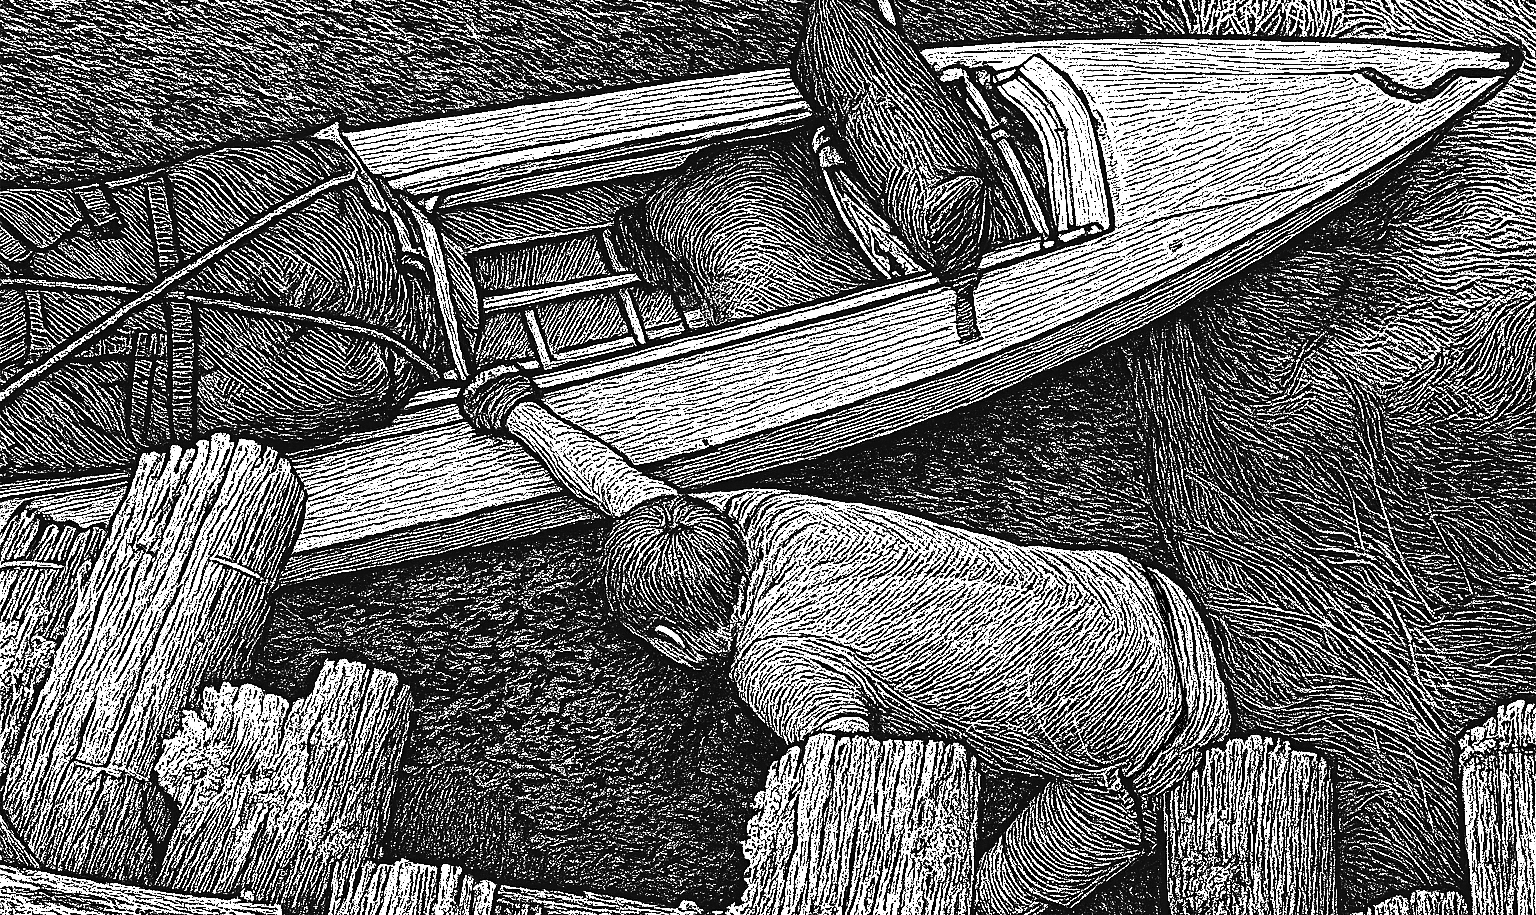
\includegraphics[width=1.0\textwidth]{22_1_serega}
	\caption{\small\textit{...Э-Э-Э!!!\mdash только и успел проорать Серёга...}}
\end{figure}

\diagdash И не говори!\mdash все отряхнулись и пошли вслед за~Адмиралом по мосту к другому берегу, проводка их взбодрила после долгого сидения в байдарках.

%\newpage
Замполит, пройдя по заливчику, причалил рядом с~шуриковой байдой. Все собрались в кружок на полянке, Адмирал раздал батончики спортпита подкрепиться:

\diagdash Подзаправимся, половину реки прошли.

\diagdash Дальше всё гладко?\mdash поинтересовалась команда.

%\renewcommand*{\thefootnote}{\arabic{footnote}}
\renewcommand*{\thefootnote}{\fnsymbol{footnote}}
\setcounter{footnote}{0}
\diagdash Как пойдёт$\ldots$\mdash протянул своё любимое Адмирал, глянув на часы.\mdash Уже около 15 часов, а нам ещё вторую половину Нурмиса пройти надо и второй мост преодолеть.\mdash сказал он, убирая карту в свой командирский планшет.

\diagdash Ладно, щас чаёк допьём и погнали.\mdash Замполит налил ещё чай из термоса и доел батончик.\mdash Чуть не~утопили байду мою, блин!

\diagdash Да не гони, всё нормально! Серёгу только подрастянули немного. Серёг, как растяжка?\mdash Адмирал допил чай и пошёл готовиться к отплытию.

\diagdash Растяжка зашибись, как выяснилось$\ldots$\mdash устало отозвался тот.
%\pagebreak

Спустя пару минут ребята, отдохнув, отчалили и пошли дальше по~петляющей среди низких топких берегов речушке. Где\sdash то примерно через километр им встретилось свежее стояночное место:

\diagdash Шурик, гляди\mdash единственное пока что стояночное место за всю речку.\mdash оживился Замполит.

\diagdash А я читал, что стоянок вовсе нет.

\diagdash Ну, кто\sdash то, похоже, психанул и решил встать лагерем прямо тут.\mdash ребята прошли мимо стоянки, на которой, судя по всему, кто\sdash то совсем недавно стоял.

Команда в спокойном режиме двигалась вперёд по~Нурмису навстречу Линдозеру. Адмирал был в~приподнятом настроении\mdash ему казалось, что дело, как говориться, в шляпе\mdash половину пути прошли, сейчас вот ещё последний мост и скоро долгожданное озеро. Но~тут из\sdash за очередного поворота донёсся оглушающий шум, даже можно сказать рёв, воды:

\diagdash Полундра! Зачаливаемся к левому берегу!!!\mdash проорал Адмирал.

\diagdash Шурик, ты угораешь?! Тут заросли!\mdash отозвался Замполит, но, быстро поняв, что тот не шутит, тоже пристал к заросшему берегу.

Ребята вылезли\mdash Адмирал знал, что тут, судя по~старой топокарте, должен быть разрушенный мост, но он никак не ожидал, что здесь окажется вполне себе полноценное препятствие, причём достаточно узкое. Серёга и~Руслан остались сторожить байды, а Адмирал с~Замполитом и Пашей отправились на~просмотр. 

Хоженой тропы для осмотра не было\mdash это обескураживало Адмирала. В~таких местах, по обыкновению, часто протаптываются хорошие добротные тропы вдоль реки, где сплавщики ходят просматривать пороги перед прохождением. Тут же ничего этого не было, им пришлось придираться сквозь плотные заросли, в которых почему\sdash то было полно паутины:

\diagdash Тьфу ты!\mdash ругался Адмирал в очередной раз напоровшись головой на паутину.\mdash Проклятье! Что~за~паучье место?!

\diagdash Шурик, что за???\mdash Киря тоже плутал среди зарослей.

\diagdash Я тут тоже в первый раз, как и вы!\mdash ответил тот. Ребята наконец\sdash то преодолели путь по зарослям и~вышли к порожку. Картина, представшая их взору, была неутешительна\mdash никакого моста, естественно, не было, но~было достаточно узкое <<бутылочное горлышко>>, в~которое устремлялся с~бешеной скоростью Нурмис, становясь белым и~пенистым. И,~что самое главное, река делала поворот, поэтому просмотреть что там дальше было нельзя. 

\diagdash Чё делаем?\mdash поинтересовался Паша у Адмирала. А тот был выбит из колеи таким препятствием и паучьей тропой, стоял соображал:

\diagdash Ну, пацаны, в принципе можно попытаться провести вот тут у камней$\ldots$

\diagdash Шурик, ты поток видел?! Какой провести?\mdash Замполит балансировал на камнях, просматривая место.

\diagdash А что ты предлагаешь?

\diagdash Так идём порог или проводим?\mdash Паша насмотрелся на белую пену и ждал когда Адмирал определится, а тот стоял в растерянности. 

\diagdash Да хрен знает! Ну куда тут чалиться? И места нет, и~тут уже течение воронкой начинается. Но чёт очково идти. Давай сюда попробуем зайти, тут вроде потише течение?\mdash Адмирал показал на участок берега, где ещё не начинались такие большие камни, как дальше. 

\diagdash А потом? \mdash Замполит закурил от стресса.

\diagdash Надо попытаться провести на чалке хотя бы первую ступень, потом залезать и дальше уже не так жёстко там, насколько видать отсюда. Короче, пошли обратно, хватит любоваться!\mdash Адмирал стремительно зашагал по~зарослям назад.

Руслан с Серёгой ждали возвращения разведки:

\diagdash Ну что там?

\diagdash Попытаемся зайти в небольшой заливчик перед порогом$\ldots$\mdash неуверенно бросил Замполит.

\diagdash Так, Паш, Руслан, давайте! Мы первые.\mdash Адмирал занял место в корме и начал отходить, табаня, против течения.\mdash Морально готовимся ко всему!

\diagdash Саня, мать-перемать! Не нравится мне это!!! Чё ты делаешь?\mdash Паша уселся и тоже начал табанить.

\diagdash Так, стоп, парни! Проворонили момент!!!\mdash ускоряющееся течение стало разворачивать байдарку поперёк реки.\mdash Криво входим!!!\mdash у Адмирала похолодело внутри.

\diagdash А-А-А!!!

%\renewcommand*{\thefootnote}{\arabic{footnote}}
\renewcommand*{\thefootnote}{\fnsymbol{footnote}}
\setcounter{footnote}{0}
Адмирал понял, что уже ни о каком зачаливании перед порогом речи не идёт, табанить тоже уже было бесполезно\mdash такую силу течения не перегрести даже втроём. Осознав, что единственный вариант это идти напролом и дальше только уповать на удачу, он круто заколол\footnote{Закол\mdash приём гребли, при котором лопасть весла забрасывается со значительным наклоном корпуса гребца в сторону весла в зону противоположного направления скорости воды под небольшим углом и~жёстко удерживается в ней.} веслом по правому борту, выправив курс, и байдарка нырнула в порог$\ldots$ Адмирал, оказавшись на сливе, ощутил вместо прежней паники уверенность\mdash они ровно вошли в~слив и~стремглав помчались дальше. Молниеносно преодолев первую ступень, он заорал:

\diagdash ПРАВЫЙ НАХОД!

Пацаны внезапно слаженно отгреблись, никто не~перепутал что и куда грести, Адмирал был доволен. Стараясь держаться середины русла, они выгребали за~поворот, Адмирал скомандовал:

\diagdash ТЕПЕРЬ ЛЕВЫЙ НАХОД, ЖЁСТЧЕ!\mdash а сам, тем~временем, оттабанил справа, и их корабль прошёл поворот русла и остаток порога.

\diagdash Прошли, мужики!!!\mdash Адмирал был вне себя от~распирающих его эмоций.\mdash Офигеть красиво!!!\mdash он просто упивался восторгом от стихии и слаженных действий своего экипажа.

\diagdash Вроде без повреждений?\mdash осматривал Паша трюм под ногами.

\diagdash Толчков в днище не было, я не заметил.\mdash Адмирал прижимался к берегу, чтобы тормознуть и подождать второй экипаж.

\diagdash А мне понравилось, вообще по кайфу прошли!\mdash Руслану пришлось по вкусу приключение.

\diagdash Пацаны, вёслами за берег зацепитесь, вылезать не~будем, ждём Кирю.\mdash Адмирал обернулся и прислушался, но не услышал никаких признаков приближения второго экипажа, рёв воды всё заглушал$\ldots$

\vspace{0.5cm}
$\ldots$Серёга с Кирей решили поступить как и~договаривались\mdash провести байду на чалке через первую ступень. Это далось им с огромным трудом, Замполит уже искупался чуть не~по~пояс. Преодолев первый, самый сильный слив, ребята решили сесть в байду и идти дальше напролом, поскольку адмиральский экипаж видно не было\mdash стало быть, те~прошли нормально. Им удалось забраться обратно в~байдарку посреди бушующего водного потока и~дальше продолжить прохождение:

\diagdash СЕРЁГА!!! ЛЕВЫМ!!!\mdash заорал Замполит, но~опоздал\mdash они~напоролись на~камень и~их~стало разворачивать мощнейшим потоком поперёк реки.

\diagdash Я И ГРЕБУ НАЛЕВО!!!

\diagdash ДА НЕ НАЛЕВО!!! А ЛЕВЫМ!!! НАОБОРОТ!!!

\diagdash КАПЕЦ!!!\mdash заорал в ответ Серёга, время было упущено, они капитально влипли.

\begin{figure}[h]
	\centering
	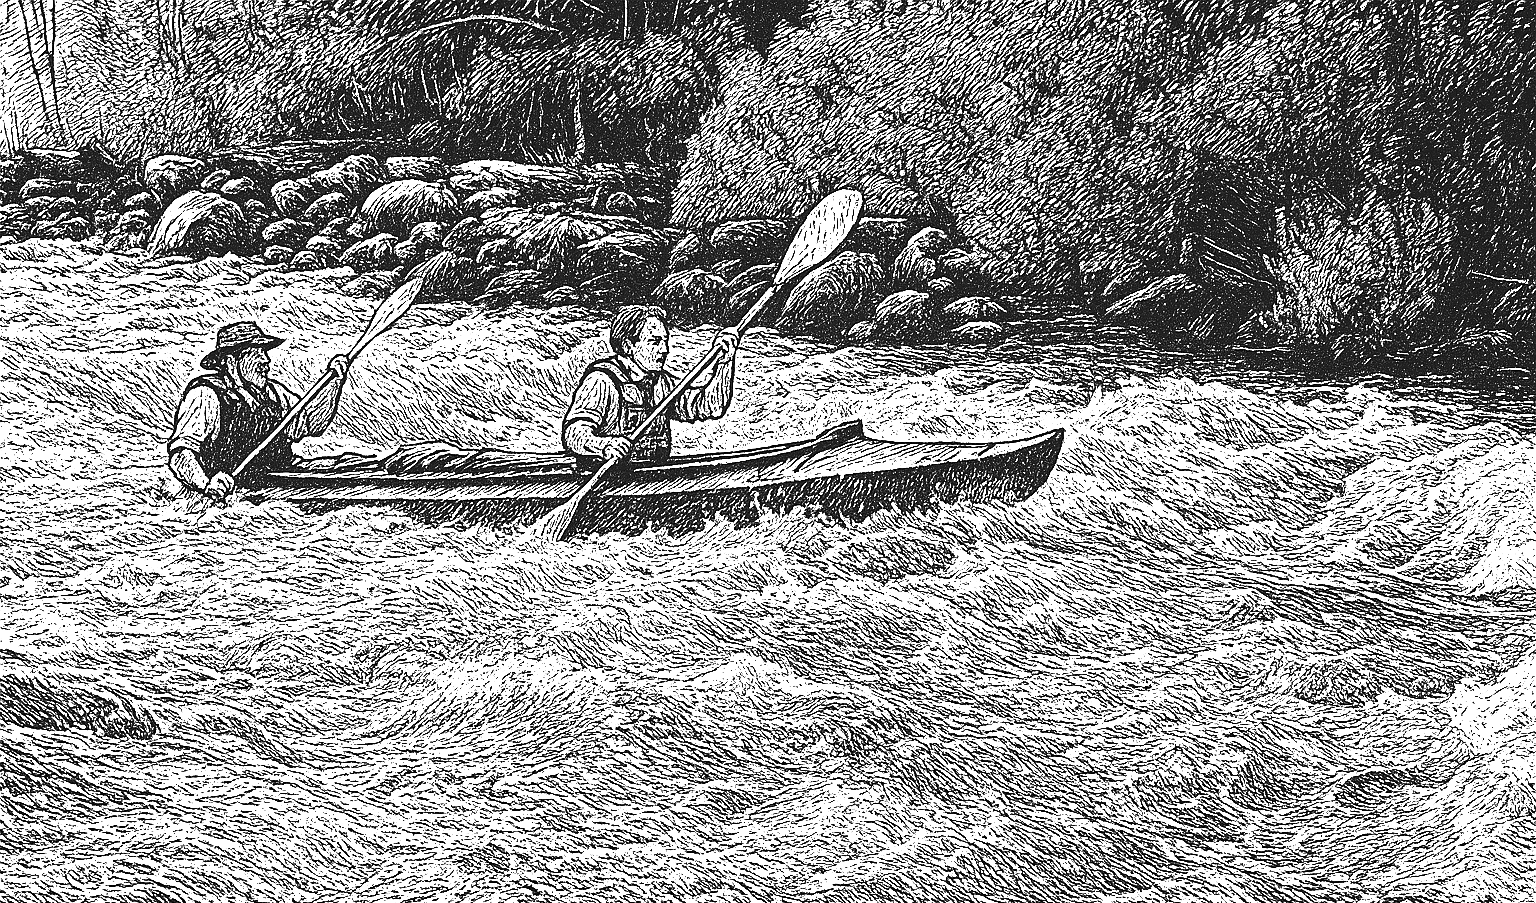
\includegraphics[width=1.0\textwidth]{23_1_fail}
	\caption{\small\textit{...Серёга!!! Левым!!!\mdash заорал Замполит...}}
\end{figure}

\diagdash Спокуха!!!\mdash Замполит жёстко отгрёбся по одному борту, и их стянуло с камня водным потоком, развернув против течения.\mdash Щ\sdash щ\sdash щас всё будет!!!\mdash упахивался он веслом, исправляя положение$\ldots$

\vspace{0.3cm}
$\ldots$Адмирал начал уже переживать за судьбу второго экипажа, сожалея, что не сказал им включить рацию, и~тут те, спустя пару минут, стремительно вылетели из\sdash за поворота кормой вперёд, совершая одновременно разворот на $180\degree$ по~курсу\mdash носом вперёд:

\diagdash Е-е-е!

\diagdash У-ху-ху!

\diagdash Ура, прошли!!! Как вы?\mdash прокричал Адмирал.

\diagdash Шурик, это подстава! Вы куда усвистели??? Договорились же проводить!\mdash Киря, негодуя, пронёсся ниже по течению.

\diagdash Отталкивайтесь от берега, парни, догоняем их!\mdash сказал Адмирал своему экипажу, оттолкнулся веслом, и они устремились вслед за~Замполитом.\mdash Ну так уже вышло, что утянуло в порог, мы бы не смогли зачалиться перед ним уже!\mdash оправдывался он Замполиту,\mdash Ладно, рассказывай как сам прошёл?

\diagdash Да мы на камень сели!!! Я ему ору: <<ЛЕВЫМ!!!>>, а~он~правым!!! Я~ему: <<ЛЕВЫМ!!!>>, а~он~правым!!!\mdash Киря обвинял матроса в~саботаже.

\diagdash Так надо говорить или с какой стороны грести, или куда ты плыть хочешь, я не понял нифига чё надо!!!\mdash отбивался яростно Серёга.

\diagdash Да ёпрст!!!\mdash Замполит чуть не скрежетал зубами на матроса, потому что ему, опытному байдарочнику, было обидно так слажать на первом же пороге.

\diagdash Забейте, пацаны, прошли и ладно, чё вы. Приспособитесь!\mdash Адмирал грёб размеренно и~воодушевлённо\mdash ему даже понравился порожек.

\diagdash Шурик, эта хрень была на карте?!\mdash спросил Серёга.

\diagdash Да, была. Только обозначена была как разрушенный мост, а~в~описании я~не~помню, чтобы на Нурмисе о чём\sdash то таком писали.

\diagdash Да ты и описание маршрута забыл!!!

\diagdash Так, аллё! Это бунт? Завязывайте давайте, прошли и~нормальды! Больше до Линдозера тут нет ничего.

Как же он ошибался! Спустя минут 40 они подошли к~очередному порожку. Адмирал был несколько обескуражен картиной. Экипажи зачалились, вылезли. Было уже около 18~часов, усталость начала накатывать волной.

\diagdash Шурик!!! Что это за???\mdash Серёга вылезал на берег.

\diagdash Нету этого порога на моей карте! Без паники, пошли на~просмотр.\mdash Адмирал вылез из байды и аккуратно вскарабкался на большие камни, грудой нараставшие по~правому берегу среди сплошных прибрежных зарослей подлеска и~густой сочной травы.

Адмирал с Замполитом скакали по камням, держа вёсла в руках. Паша тоже пошёл с ними, Руслан и~Серёга опять остались у~байдарок. Взору разведчиков открылся порожистый участок длиной метров 200. Дело ухудшалось тем, что проход по воде был очень узким, простора для манёвра не было никакого, Адмирал опешил.

\diagdash Это полная задница!\mdash Замполит сновал по камням.

\diagdash Пошли дальше просмотрим?\mdash Паша устремился вперёд через заросли прибрежной травы и камни. Парни пошли, перелезая по огромным валунам, вдоль берега дальше, стремясь не ломануться в воду с качающихся серо\sdash чёрных камней.

\diagdash Мда-а-а, пацаны.\mdash Адмирал немного растерялся. Он уже не ждал никаких сюрпризов от Нурмиса и вот тебе. Обноситься тут было вообще кошмарно\mdash он как представил, что по этим камням тащить байду на плече, а~потом и~все шмотки, гермы, вещмешки, так сразу и убрал эти мысли подальше. Надо было проходить по воде, это стало очевидным. Но~как? Он дико сомневался в том, что под этой коварной водной гладью не скрываются камни. Ребята пробрались примерно к середине порога:

\diagdash Так, мужики, ну вот. Отсюда более менее видно всё. Пройти по центру можно. И нужно. Гляди, Паш,\mdash Адмирал показывал руками,\mdash вот тут уходим правее, потом левее, потом снова правее$\ldots$

\diagdash А успеем? Тут такое же течение, как и в прошлом пороге, пикнуть не успеешь.\mdash перебил Паша, сомневаясь.

\diagdash В целом, я думаю, только вход важен\mdash во-о-он тот камень обойти,\mdash Адмирал показал рукой,\mdash и дальше уже по ситуации, всё равно мы с берега не увидим всей картины, что будет на воде.

%\newpage
\diagdash Короче первый камень обходим справа, дальше надо левее взять, а потом уже по ситуации, походу, змейкой такой.\mdash Паша проговаривал стратегию с Адмиралом. 

\diagdash Это полная задница!\mdash повторил Замполит. Ему~в~принципе не~нравилась идея ломиться по такому узкому руслу, лавируя меж камней.

\diagdash Ты ж бывалый походник, ё-моё! Карелия, Кереть, третья категория там, и~прочее! Чего раскис?\mdash Адмирал старался приободрить Замполита.

\diagdash Шурик, знаешь чё?!\mdash Киря был в упадническом настроении.

\diagdash Знаю! Ничего больше мы тут не увидим, пошли обратно!\mdash сказал вдруг Паша, и они засобирались к~остальной части команды, которая порядком притомилась, ожидая возвращения разведки. Издалека было видно, как Серёга с Русланом тоже стояли у начала порога и что\sdash то махали руками, показывая на русло.

Спустя пару минут разведчики вернулись, аккуратно ступая по камням, и забрались на возвышение у начала порожка:

\diagdash Ну что?\mdash Серёга с Русланом ждали тех с~нетерпением.

\diagdash А что? Идём!\mdash ответил Адмирал.\mdash На этот раз включи рацию, Кирь, я тебе расскажу как и что, когда пройду, чтоб связь была!\mdash сказал он, повернувшись к~Замполиту. Тот достал рацию из гермы:

\diagdash Куда жать, Шурик?

\renewcommand*{\thefootnote}{\arabic{footnote}}
%\renewcommand*{\thefootnote}{\fnsymbol{footnote}}
\setcounter{footnote}{0}
\diagdash Вот громкость,\mdash показал Адмирал на верньер\footnote{Верньер в радиотехнике\mdash приспособление для тонкой настройки, обычно выполняемое в виде круглой рукоятки.},\mdash а~вот тангента\footnote{Тангента\mdash кнопка или клавиша переключения с приёма на передачу на радиостанции.} сбоку. Жмёшь на неё и говоришь. Всё~просто! Кнопки другие не нажимай, настройки не меняй, всё работает. Давайте, погнали!

Адмиральский экипаж уселся в байдарку, отошёл от~берега. Нужно было отойти чуть подальше, выше по~течению, прицелиться и~ровно войти в~начало порога. Адмирал отгрёбся, выравнялся, убрал рацию в герму, сел поудобнее, перехватил весло: 

\diagdash Мужики, готовьтесь!\mdash Адмирал поёрзал, сидя на~своей герме, стараясь сесть повыше, чтобы обеспечить себе обзор получше.

\diagdash Может не надо?\mdash спросил Паша, особо не надеясь на~то, что Адмирал одумается. А тот был внешне спокоен, хотя в душе, конечно, был на диком взводе\mdash во\sdash первых, такие пороги Адмирал никогда не брал, а во\sdash вторых, он не был готов к такому сюрпризу под конец дня, однако постарался как\sdash то мобилизовать все свои силы.

%\renewcommand*{\thefootnote}{\arabic{footnote}}
\renewcommand*{\thefootnote}{\fnsymbol{footnote}}
\setcounter{footnote}{0}
\diagdash Выравниваемся, заходим!\mdash байдарка пошла вперёд, скорость была аховая.\mdash ЛЕВЫМ! ЛЕВЫМ!!!\mdash проорал Адмирал, и они стремглав успешно миновали тот камень, что больше всего не~понравился при~просмотре.\mdash НЕ~ГРЕБЁМ!!!\mdash он затабанил слева и тут же жёстко справа, чтобы S\sdash образно обойти второй обливняк\footnote{Обливной камень, или обливняк\mdash камень в русле реки, едва прикрытый водой.} по~правому борту.\mdash ТЕПЕРЬ ПОЛНЫЙ ВПЕРЁД!!!\mdash экипаж стремительно прошёл первую половину порога, их взору открылся выход и вторая половина, где были полуметровые стоячие валы. Адмиралу стало жутковато на мгновение, но~потом он воспрял и, подправив курс, заорал экипажу:

\diagdash НЕ ГРЕБЁМ!\mdash они ровно шли на валы. Миг,~и~вал поглотил нос их байдарки, Адмирал видел, как волна заливает сидящего спереди Пашку и докатывается до~Руслана. Адмиралу достались только брызги. Почему\sdash то никому, даже Адмиралу, не пришла в~голову мысль перед этим штурмом надеть байдарочные юбки, и теперь всех изрядно окатило брызгами. Сердце Адмирала сжалось от~толчка в~днище байды. <<Только бы не пробоина>>,\mdash подумал он. Секунда, и второй вал окатил их, потом третий$\ldots$ Адмирал~держал~курс,~они~пробивали валы. Его сердце, стучащее на адреналине часто\sdash часто, даже если бы и хотело выпрыгнуть из груди, всё равно бы не~успело\mdash настолько всё быстро и~молниеносно произошло. 

Наконец, последний вал остался позади, ребята проскользили выход из порога. Вода успокоилась, и теперь о~пороге напоминала только пена, плывущая рядом. Адмирал заложил правый поворот, следуя изгибу петляющей реки:

\diagdash Й-й-й-и-и-ха!\mdash орали они.

\diagdash Прошли!!!

\diagdash Да!!! А-А-А!!!\mdash радовался Адмирал.

\diagdash По\sdash моему, пару толчков в днище всё таки было.\mdash сказал, обернувшись назад, Паша. 

\diagdash Да, я тоже почувствовал,\mdash отозвался Адмирал.\mdash Ты как, нормально?\mdash спросил он у Руслана.

\diagdash Вообще по кайфу!!! Дольше, по\sdash моему, обсуждали это~всё!

\diagdash Да, есть такое$\ldots$ Так, мужики, давайте, правый табан, левый наход, встаём против течения у правого берега в кустах, ждём второй экипаж.\mdash они встали в области обратного течения после порога и зацепились вёслами за~берег.

Адмирал достал рацию:

\diagdash Кирь, мы прошли нормально, как слышно меня? Приём.\mdash и~отпустил тангенту.

\diagdash Слышно хорошо, а что пиликает?\mdash отозвался Замполит по рации.

%\renewcommand*{\thefootnote}{\arabic{footnote}}
\renewcommand*{\thefootnote}{\fnsymbol{footnote}}
\setcounter{footnote}{0}
\diagdash Это роджер\footnote{Роджер (англ. roger)\mdash одно- или двухтоновый сигнал, автоматически выдаваемый рацией в эфир при переключении с передачи на приём.}, забей. Короче, мы прошли нормально, главное обойти первый камень справа, а дальше более\sdash менее как по маслу, днищем слегка цепанули, но пробоины вроде нет. Мы вас за поворотом ждём. Приём!

\diagdash Шурик, мы пешком пойдём, я не вижу куда плыть в~этой каше. Приём!

\diagdash Ты угораешь?! Я говорю, нормально прошли мы, главное обливняк обходи и всё. Как понял? Приём!

{
\setlength{\belowcaptionskip}{-20pt}
\begin{figure}[h]
	\centering
	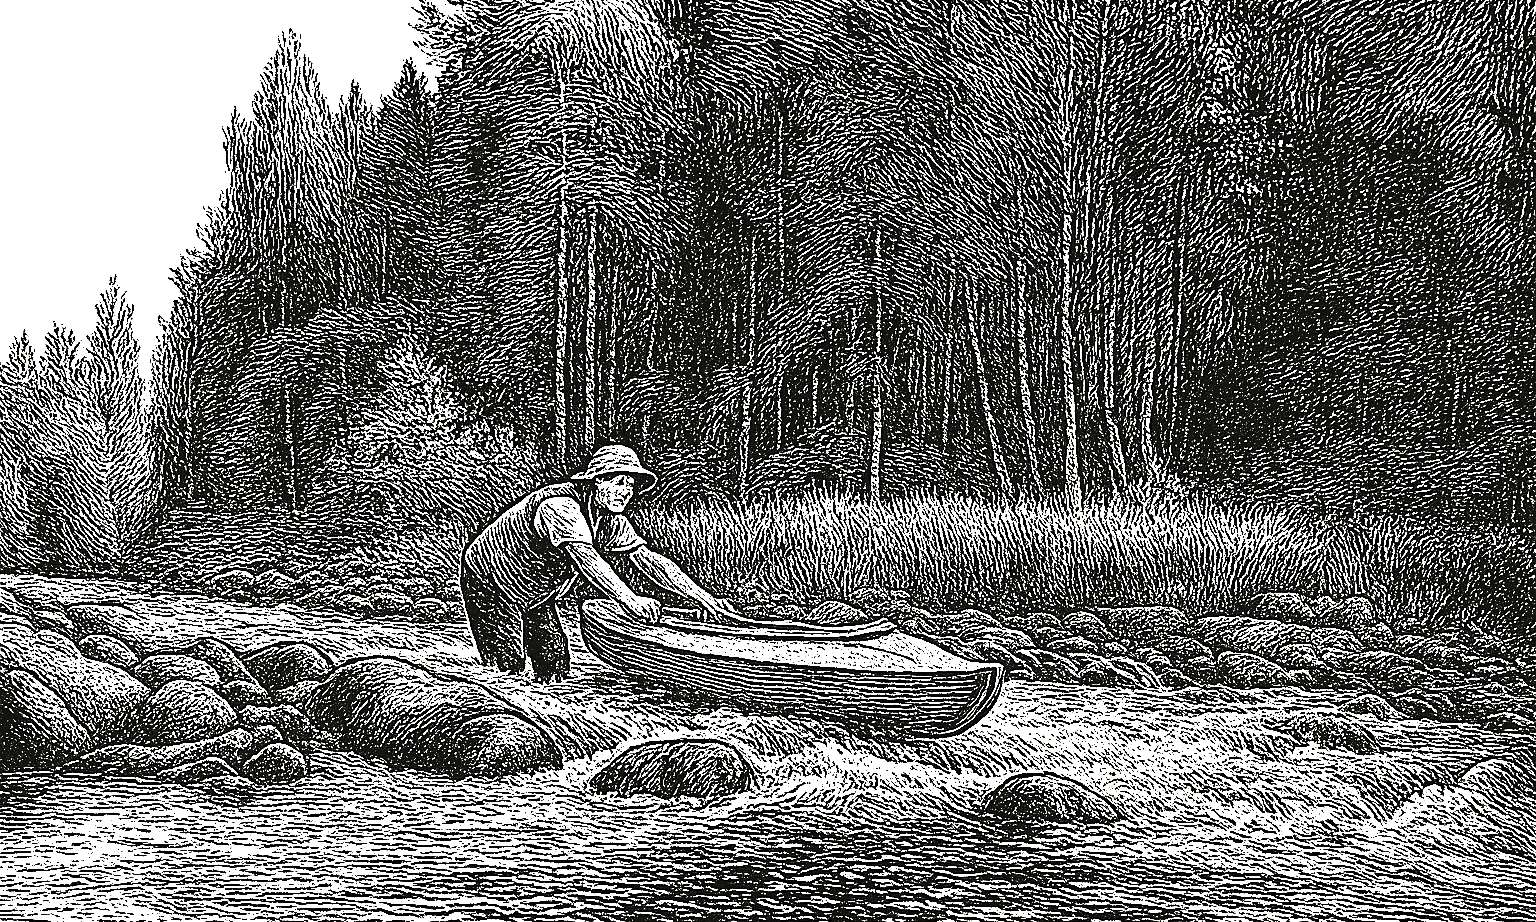
\includegraphics[width=1.0\textwidth]{24_1_nurmis}
	\caption{\small\textit{...пошли проводиться...}}
\end{figure}
%
\diagdash Я понял, Шурик, мы не пойдём, будем проводить на~чалке, я~нифига не хочу сейчас клеиться! %\mdash он боялся распороть байдарку о камни.
}

\diagdash Не делай м\'{о}зги, мы просквозили почти что на чиле! Давай жми!

\diagdash Ты времени видел сколько? Нам еще полпути, а мы в какой то заднице застряли! Прикинь щас полборта клеить? Всё, мы пошли пешком$\ldots$

Адмирал охренел от внезапного замполитовского демарша, уж Киря\sdash то не должен был испугаться идти порог:

\diagdash Кирь, давай не делай мозги, мы прошли нормально, я те говорю! Приём!

\diagdash Мы пошли проводиться берегом, ждите$\ldots$

Адмирал грязно выругался, отложил рацию, поняв, что спорить бесполезно, и сказал своему экипажу:

\diagdash Ну, вы слышали, парни. Чилим, ждём их.

\diagdash Ладно, тогда посмолим, что ли.\mdash Пашка достал трубку и стал её чистить.\mdash Давненько не пользовался$\ldots$

\diagdash Ну что ты будешь с ними делать, а?\mdash Адмирал раздосадованно достал портсигар и задымил. Руслану ничего не оставалось, как тоже смолить и ждать. И они, держась вёслами за~берег, ждали. Пашка закончил чистку трубки и~задымил, попытавшись откинуться на спинку шпангоута:

\diagdash Красотень, натурально!

Адмирал достал навигатор и решил промерить, раз всё равно пока делать было нечего, сколько им ещё осталось пройти\mdash точная информация о километраже всегда положительно действует на командный дух, он знал это по~опыту. Оказалось, что по Нурмису осталось пройти всего\sdash то около двух километров, а~дальше начиналось Линдозеро. Забавляло, что многие карельские названия озёр включают в себя само слово <<озеро>>, что является калькой с финского\mdash <<ярви>>, <<jarvi>>. То же относится и~к~прудам или маленьким озёрам\mdash <<лампи>> и другим географическим объектам. Почему так вышло\mdash уже дело тёмное. Скорее всего, в~20\sdash е или 30\sdash е годы XX века, на~заре советской власти, в~эпоху заигрывания с~национальными республиками, так решили. Но факт остаётся фактом\mdash <<Lindjarvi>> трансформировалось путём дословного перевода в <<Линдозеро>>, и получилось масло масляное\mdash <<озеро~Линдозеро>>. Собственно, на~старой адмиральской топокарте так и было отмечено\mdash <<оз.~Линдозеро>>. 

Адмирал сидел и рассматривал это самое озеро на~топокарте и прикидывал, что по~нему ещё километра полтора пройти придётся до~архипелага островов посередине. Ему непременно хотелось встать лагерем на~днёвку на~острове, это как бы само собой подразумевалось, и никакой другой стоянки Адмирал в~принципе не мыслил.

Пашка всё ещё дымил, а Адмиралу наскучило ждать, он попытался связаться со вторым экипажем по рации, но~те~не~отвечали. Ребята умаялись ждать, и у Адмирала, который расслабился было после прохождения порога, вновь стало нарастать чувство тревоги, он даже уже подумал, что надо бы отойти от берега и выйти к порогу против течения, посмотреть что там с Серёгой и Кирей:

\diagdash Чё, может сходим посмотрим где они?

\diagdash Да ладно, щас придут.\mdash Паша сидел смолил трубочку, расслаблялся.

\diagdash Мы вроде по кайфу просквозили, наверно они тоже?\mdash Руслан перезацепился веслом за берег.

\diagdash Хотелось бы верить$\ldots$\mdash отозвался Адмирал.

Прошло уже около сорока минут, когда из\sdash за поворота наконец\sdash то появился второй экипаж:

\diagdash Пацаны, вы угораете?! Чё вы не пошли за~нами\sdash то?!\mdash злился Адмирал.

\diagdash Шурик, остынь, мы бы не прошли уже с Серёгой эти валы.\mdash пытался оправдаться Замполит.

\diagdash Да всё б вы прошли, зассали! Ладно, не утопли, и то хорошо. А то я тут курю и переживаю, курю и переживаю!

\diagdash Шурик, мы задолбались пешком проводить, не~прессуй.\mdash Серёга выглядел уставшим.

{
\diagdash Вот перекурить не мешало бы.\mdash заметил Замполит.

%\diagdash Кирь, <<привет>> от пульмонолога!\mdash подколол того Адмирал.
\diagdash <<Привет>> от пульмонолога!\mdash подколол Адмирал.
}

\diagdash Шурик, иди\sdash ка$\ldots$?

\diagdash Ы\sdash ы\sdash ы!

\diagdash Хочешь сказать, этого не было на карте?!\mdash Серёга был, естественно, не в восторге от тяжёлого волока.

\diagdash Было$\ldots$\mdash сознался Адмирал,\mdash Но обозначено было как <<зимник>>. Так что, как бы, без обид.

\diagdash Зимник, едрить! Да это целый порог!\mdash Серёга всё никак не мог уняться.

\diagdash Да какой порог, так, шиверка небольшая. Мы~с~б\'{о}льшей осадкой, чем вы, да и на трёшке неповоротливой, и то прошли, а вы, блин!\mdash Адмирал не стал больше придираться ко второму экипажу, и они вместе пошли дальше. 

Спустя три или четыре следующих друг за другом резких поворота реки они увидели огромную рыбацкую стоянку\mdash там был причал, небольшой домик типа сарая, состоящий из комнаты с печкой и террасы. Место было обжитым и замусоренным. Команда разбрелась по берегу, все вытащили термосы с чаем, решили немного передохнуть, размять ноги.

\diagdash Что это за место?\mdash спросил Руслан.

\diagdash Похоже на рыбацкую стоянку. Причал хороший, избушечка тоже. Вероятно сюда с Линдозера, с~деревни в~смысле, народ приплывает на заготовку рыбы, ягод. Похожие избы в тайге охотники ставят, только там, конечно~же, мусора меньше. Культура, мать их за~ногу!\mdash Адмиралу было досадно, что такое красивое место с избушкой испорчено всякими банками, бутылками, пластиком и~полиэтиленом.

\diagdash Оставаться здесь\mdash не круто.\mdash заключил Замполит, смачно затянувшись сигареткой, прогоняя недавний стресс.

\diagdash Однозначно.\mdash подтвердил Адмирал.\mdash Мы лучше на~острове встанем, как Робинзоны.

Пашка изучал огромную гору рыбьей чешуи:

\diagdash Красота, рыбы\mdash завались. Кто\sdash то недавно ушёл отсюда, походу.

\diagdash Нам тоже пора. По коням, пацаны!\mdash Адмирал пошёл отвязывать чалку.

Остаток Нурмиса был совсем непримечателен. Сплавщикам вскоре открылся вид на раздвоение русла\mdash направо уходил короткий канал к озеру, и~они завернули~в~него.

\diagdash Шу-у-урик, опять канал?\mdash спросил Серёга.

\diagdash Ага! Последний, больше точно не будет! Ха!

\diagdash А этот\sdash то зачем прорыли? 

\diagdash Ну, он сокращает путь из реки в озеро и обратно\mdash там на развилке если левее было идти, как по руслу историческому, там дальше петляние пойдёт и, я~подозреваю, мель. А тут\mdash хопа!\mdash сразу в озере оказываешься. Удобно,~ну?

Эскадра прошла канал, их взору открылся простор Линдозера. Времени было уже к двадцати часам, оранжевое закатное солнце начало склоняться над соснами. Адмирал~сверился~с~навигатором и повёл эскадру прямо вперёд, к самому большому острову посреди озера. Когда ребята миновали мыс справа по курсу, то увидели, что на~меньшем острове справа стояли байдарочники\mdash было издалека видно штук семь ярких плавсредств:

\diagdash Так, маленький остров забит.\mdash резюмировал Адмирал.\mdash Паш, ветер попутный! Ставь парус!!!

\diagdash Ага!

\diagdash И чуть левее правим!\mdash скорректировал Адмирал курс после прохождения маленького острова справа по борту.

Ветер стремительно тащил их вперёд к острову, западная оконечность которого привлекала издалека, полоска жёлтого пляжа так и манила к себе. Парус отлично тянул адмиральскую трёшку, а вот грести сил уже оставалось мало\mdash все устали, прохождение Нурмиса и~скачки по~камням отняли прилично сил. В~этот день они прошли около двадцати пяти километров.

Нос адмиральской байды на скорости зарылся в~песчаный пляж долгожданного острова, Адмирал выскочил на берег. Рядом причалил и Замполит:

%\begin{wrapfigure}[12]{r}{0.5\textwidth}
%\begin{figure}[h]
%	\centering
%	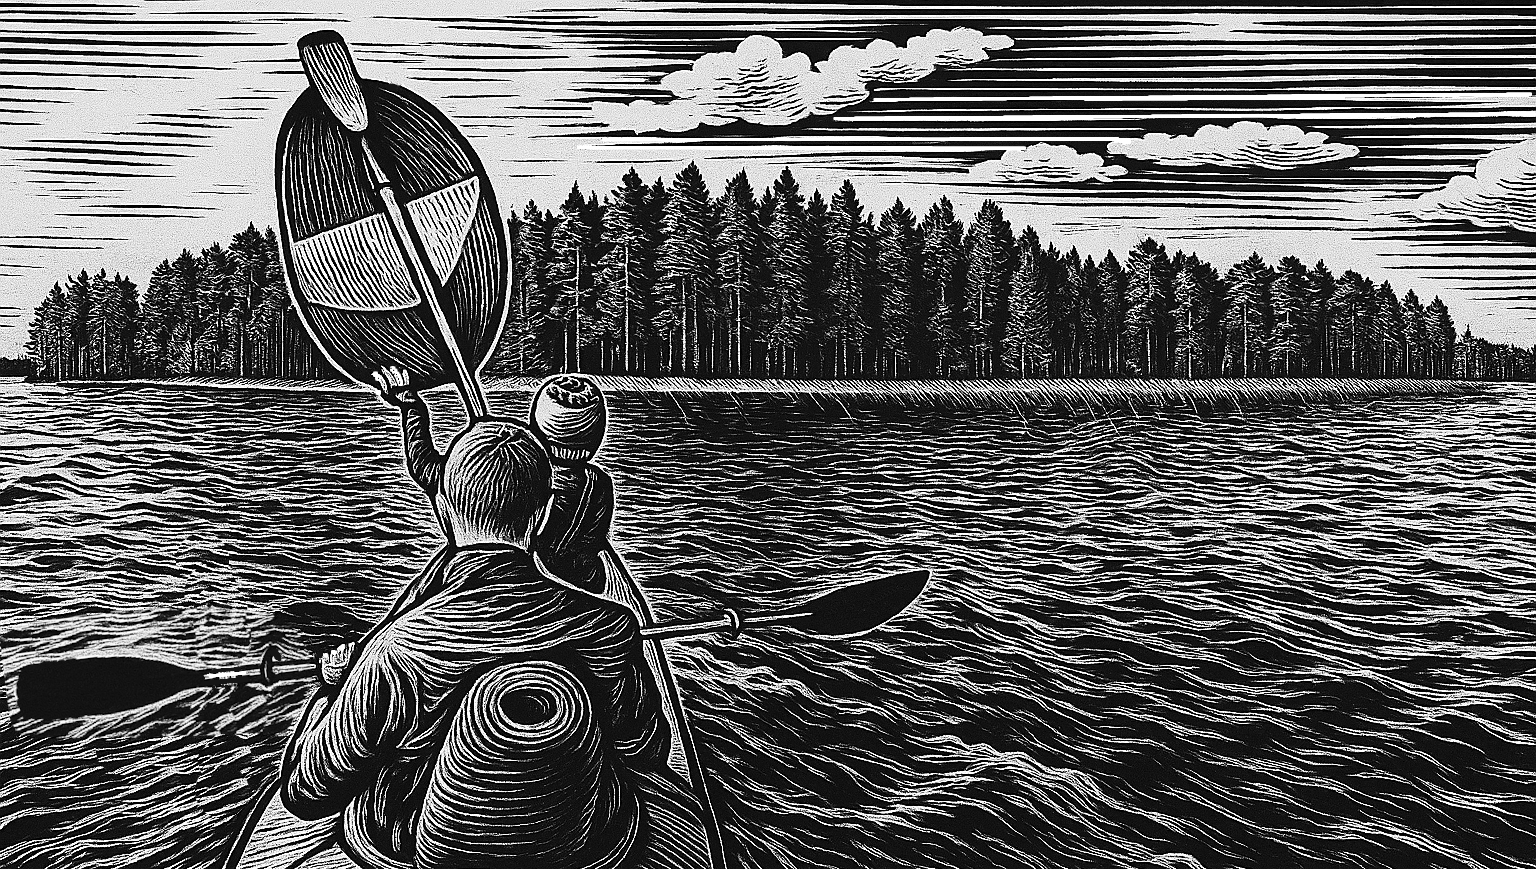
\includegraphics[width=1.0\textwidth]{9_2_new3}
%	\caption{\small\textit{...Ветер стремительно тащил их вперёд к острову...}}
%\end{figure}
%\end{wrapfigure}

\diagdash Ура-ура-ура! Ищем стояночку!\mdash воспрял он. Все~пошли на западный мыс острова, где была большая песчаная коса, уходившая, видимо, плавно дальше под воду. Ребята нашли небольшое костровище, но, в целом, место было ни~о~чём. К тому же мыс насквозь продувался приличным ветром с озера. Оранжевое солнце приветливо освещало сосны. Все~походили, пошатались, отдыхая от гребли:

\diagdash Чёт как\sdash то не аллё!\mdash Адмирал и так, и~эдак мысленно прикидывал, как тут организовать лагерь, но~ему всё не нравилось. Команда была схожего мнения. Тогда~Адмирал решил пойти вдоль пляжа в другую сторону, посмотреть там:

%%\begin{wrapfigure}[12]{r}{0.5\textwidth}
\begin{figure}[h]
	\centering
	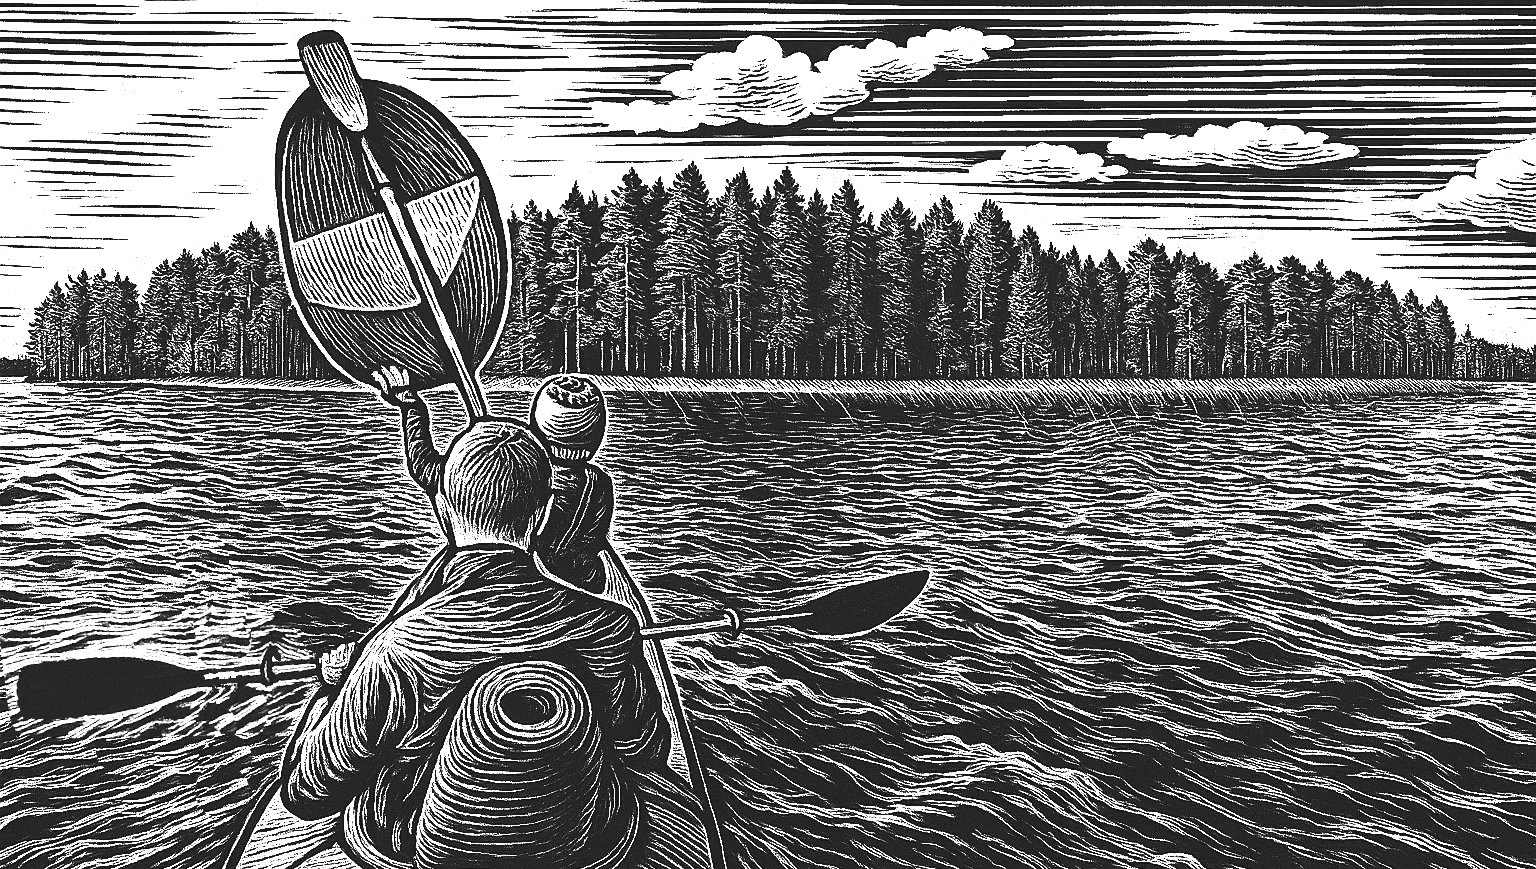
\includegraphics[width=1.0\textwidth]{25_1_island}
	\caption{\small\textit{...Ветер стремительно тащил их вперёд к острову...}}
\end{figure}
%%\end{wrapfigure}

\diagdash Пацаны, погнали там глянем?

\diagdash Пошли!\mdash отозвался Замполит. Остальные не~поддержали их энтузиазма и остались у байдарок.

Они вдвоём дошли до небольшого мыса по кромке песка. Стояночного места решительно не было. Чувство разочарования как\sdash то прямо точило Адмирала изнутри. Такой шикарный пляж был на спутниковых снимках, и вот они идут по нему в гидроносках, а стояночного места\mdash ну~никак нету.

\diagdash Шурик, совсем всё не то. Можно, конечно, теоретически, провести, как ты любишь говорить, широкомасштабные шанцевые работы, но что\sdash то как\sdash то$\ldots$

\diagdash Согласен, Кирь, тем более мы, на секундочку, ищем место на днёвку. А значит, я хочу, как минимум, шикарный пляж, шикарное костровище и шикарный лес.\mdash они уже шли обратно с решением отчалить и искать стоянку дальше.\mdash По~коням, парни! Идём дальше!\mdash скомандовал всем Адмирал.

\renewcommand*{\thefootnote}{\arabic{footnote}}
%\renewcommand*{\thefootnote}{\fnsymbol{footnote}}
\setcounter{footnote}{0}
Эскадра встала на воду, Паша свернул парус, поскольку с ним можно было идти только при попутном ветре, а они шли левым галфвиндом\footnote{Галфвинд (англ. halfwind\mdash полветра)\mdash курс парусного судна относительно ветра, когда угол между диаметральной плоскостью судна и направлением ветра составляет $90\degree$\cite{МорскойСправочник}.}. Нужно было обогнуть западную оконечность острова, там где была песчаная коса. Коса, как выяснилось, далеко уходила под воду дальше. Там~было мелко, и в этом месте рос тростник, торча из воды. Команда напоролась на мелководье с топким вязким песком. Адмирал~попробовал~вылезти~из~байды и оттолкнуться ногой, но она ушла в зыбучий песок:

\diagdash Попадос, парни! Копаем вёслами активно! Отталкивайтесь от~песка!!!

\diagdash А если мель большая?\mdash засомневался Серёга.

%\renewcommand*{\thefootnote}{\arabic{footnote}}
%\renewcommand*{\thefootnote}{\fnsymbol{footnote}}
%\setcounter{footnote}{0}
\diagdash Не должна$\ldots$\mdash Адмирал был уверен, что песчаная полоса узкая.\mdash Уваливаемся вправо на фордевинд!\footnote{Фордевинд (гол. voordewind)\mdash курс судна, совпадающий с~направлением ветра\cite{МорскойСправочник}.}

Спустя несколько минут адской борьбы с песчаной мелью, они вышли из тростника на глубину:

\diagdash Уф\sdash ф\sdash ф! А всего\sdash то надо было чуть подальше отойти и там бы спокойно прошли, а?\mdash сказал раздражённо Паша.

\diagdash Это не наш стиль! Забей, идём дальше!\mdash Адмиралу уже дико хотелось найти стояночное место вот прям сейчас. 

Они шли параллельно северной стороны острова примерно в~ста метрах от берега. Берега были откровенно никакими, стоянок не просматривалось, даже на разведку причаливать не было желания. Адмирал нет\sdash нет, да~и~посматривал на~северный берег озера\mdash до него было около километра и просматривалось редколесье, впрочем, тоже ничего не гарантирующее в плане хорошей стоянки:

\diagdash Парни, у кого там подзорная труба? Гляньте, чё там со стоянками во\sdash о\sdash он на том берегу?

Паша попробовал провести визуальную разведку, но~ничего толком они, конечно, не~разглядели.

\diagdash Шурик, сработал Закон Половины Восьмого\cite{Квадригин}\mdash стоянки исчезли!\mdash обречённо сказал Замполит.

\diagdash Не накаркай! Всё щас найдём! На северо\sdash восточном мысу точно есть стоянка!\mdash ответил Адмирал.

\diagdash С чего бы?

\diagdash Там место должно быть красивое и большой песчаный мыс, как треугольник, судя по спутниковым снимкам!\mdash просветил Адмирал. <<Но навряд ли оно окажется не занятым>>,\mdash подумал он. Ветер поутих, потому что они стали огибать остров с севера, и он прикрыл их.

\diagdash Красивое место, да$\ldots$ И оно занято!\mdash сказал, увидав впереди на камнях мужика, Серёга.

\diagdash Да ёклмн! Может это местный, ну с деревни?

\diagdash В цветастой туристической одежде?

\diagdash Да ёпрст!

\diagdash Идём дальше!

Ребятам пришлось лопатить дальше, чтобы обогнуть мыс, где действительно стояла лагерем большая группа с~детьми\sdash дошкольниками. Обогнув мыс и повернув на юг, они подставились встречному ветру, который вырывался из\sdash за острова на озёрный простор. Бороться с полным сильным встречным ветром стало невероятно тяжко, все напряжно гребли, упираясь.

И тут они увидели, как недалеко от занятой стоянки на мысу девушка, видимо только что искупавшись, стояла, завернувшись в одно полотенце, и расчёсывала свои длинные, чёрные как смоль слегка вьющиеся волосы$\ldots$ Она, наклонив голову, приглаживала девичье богатство\mdash шикарные копны волос, а слегка согнутая в колене обнажённая нога грациозно выглядывала из под полотенца. Команда аж перестала грести. Увидев две байдарки на воде, девушка смутилась и поправила рукой запахнутое на~статной груди полотенце. Адмирал первым нашёлся:

\diagdash Так, парни, слюну подобрали, только третий день похода, рано ещё об этом мечтать.

\diagdash Считая заброску\mdash пятый!

\diagdash Ы-ы-ы!

\diagdash Валькирия!

\diagdash Те светловолосые были$\ldots$

\diagdash А талия?

\diagdash Талии за полотенцем не видно!!!

\diagdash А ножки?

\diagdash У-лю-лю!!!

\diagdash Ничё так!

\begin{wrapfigure}[23]{l}{0.6\textwidth}
	%\begin{figure}[h]
	\centering
	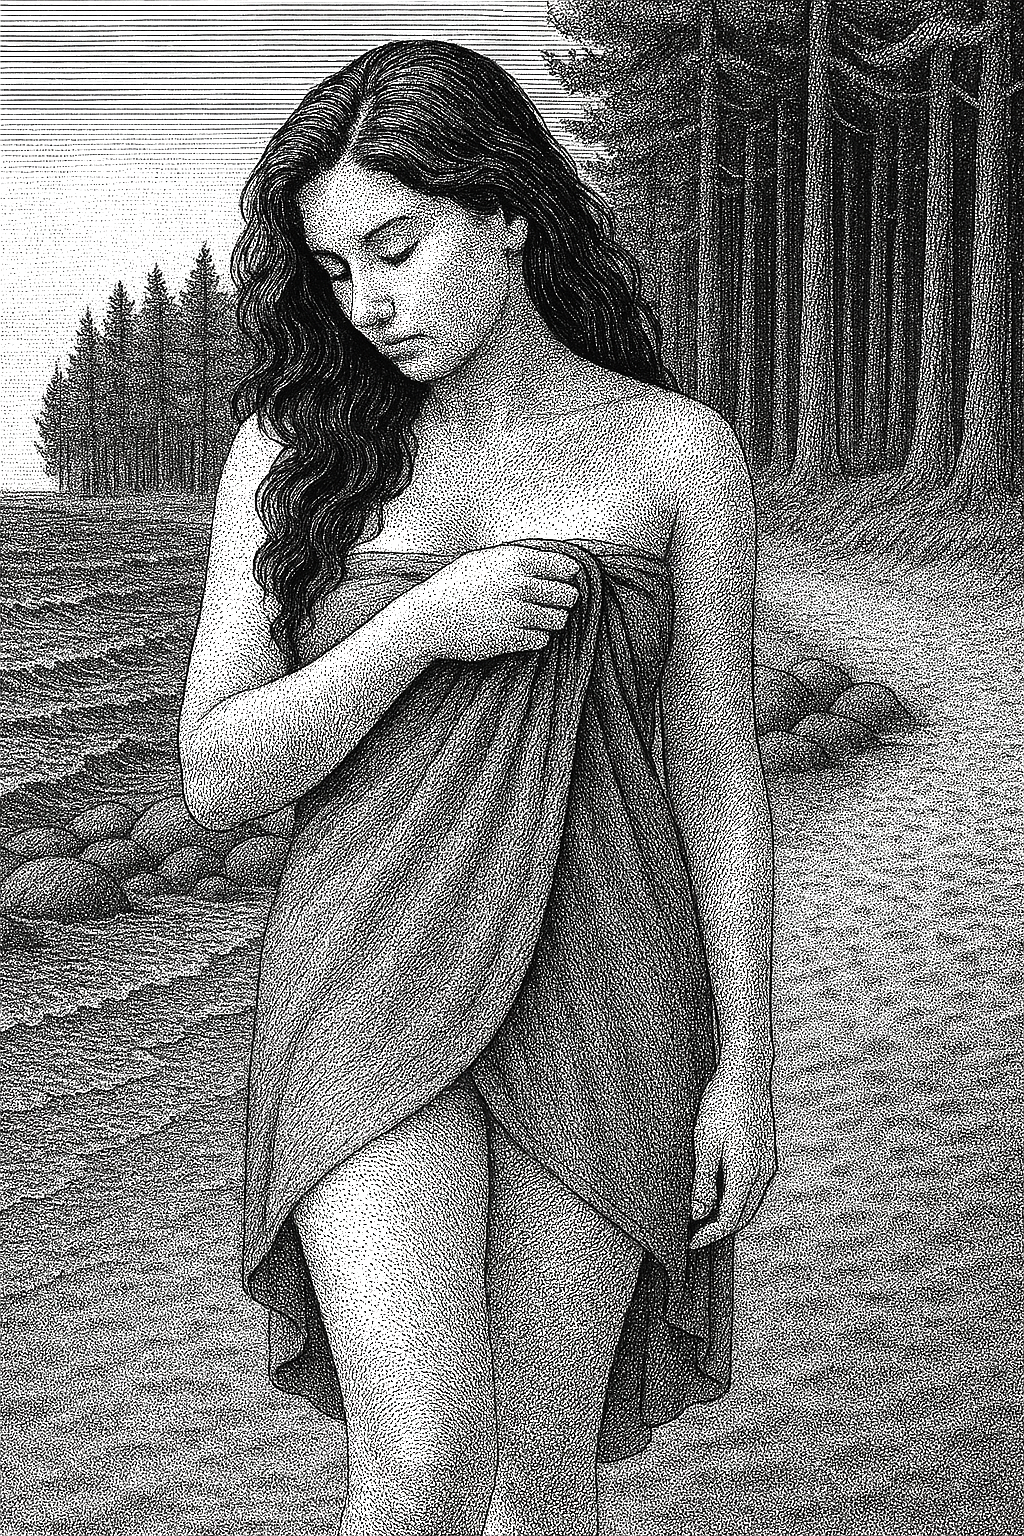
\includegraphics[width=0.6\textwidth]{26_4_valkyrie}
	\caption{\small\textit{...завернувшись в одно полотенце...}}
	%\end{figure}
\end{wrapfigure}

\diagdash Дьявол, да хар{\'о}ш уже!!!\mdash Адмирал начал грести по\sdash активнее, чтобы справиться с~нахлынувшим.

\diagdash Шурик, куда ты так гребёшь?%Дай насладиться\sdash то, ну?

\diagdash Стоянку на днёвку ищем, или мне это снится?\mdash огрызнулся Адмирал.

\diagdash Ишь ты!\mdash Киря подрезал его на повороте,\mdash Хопа!\mdash и вышел вперёд.

\diagdash В заливчике давайте поглядим!\mdash Адмирал жадно вглядывался в~берег, они обогнули южный мыс и~зашли в~небольшую бухту.

\diagdash Что\sdash то глухо, а?\mdash Серёга грёб потихонечку.

\diagdash Вон полосочка песочка! Чалимся, идём в разведку!\mdash распорядился Адмирал, увидев в глубине прибрежных зарослей подъём наверх к сосновому лесу, где проглядывался столик.

Они пристали к песчаному берегу под сосной, росшей прям у кромки озера и раскинувшей свою крону и над водой, и над берегом. Все вылезли из байдарок, размяли уставшие спины. Солнце последними тёплыми закатными лучами красиво освещало прибрежный лес. Адмирал вскинул руку со своими китайскими ролексами\mdash времени было ровно 20 часов.

\diagdash Так, парни, а вот и тропинка!\mdash Адмирал стал пробираться сквозь заросли папоротника вперёд к~подъёму.\mdash Пошли глянем, что да как!

Команда поднялась наверх и увидела старую туристическую стоянку\mdash посреди светлого высокого соснового леса располагалась большая поляна. Костровища не было, поскольку оно, видимо, успело зарасти, зато был столик и покосившиеся скамейки, настолько уже хлипкие, что сидеть на них было нельзя. Следов недавнего пребывания здесь человека не наблюдалось, мох и трава были нетронутые. Адмирал понял, что ничего лучше они сейчас уже не найдут, и велел разгружаться:

\diagdash Место на четвёрочку, возможно с минусом, но выбора уже нет, восемь вечера. Искать что\sdash то другое нет ни сил, ни~светового дня. Короче, остаёмся.

\diagdash Лад\'{ы}, погнали таскать вещи!\mdash все пошли вниз к~байдаркам.

\diagdash И это, есть уже хочется немерено, давайте в темпе всё мутим!

Ребята быстро разгрузили байды прямо у тоненькой кромки песчаного пляжа под сосной и затащили их чуть поодаль в папоротник, предварительно нафоткавшись в~последних тёплых лучах заходящего солнца. Пляжик был обращён на юг, то есть как раз на них дул ветер с~озера, но сейчас, под ночь, он стих.
%\begin{figure}[h]
%	\centering
%	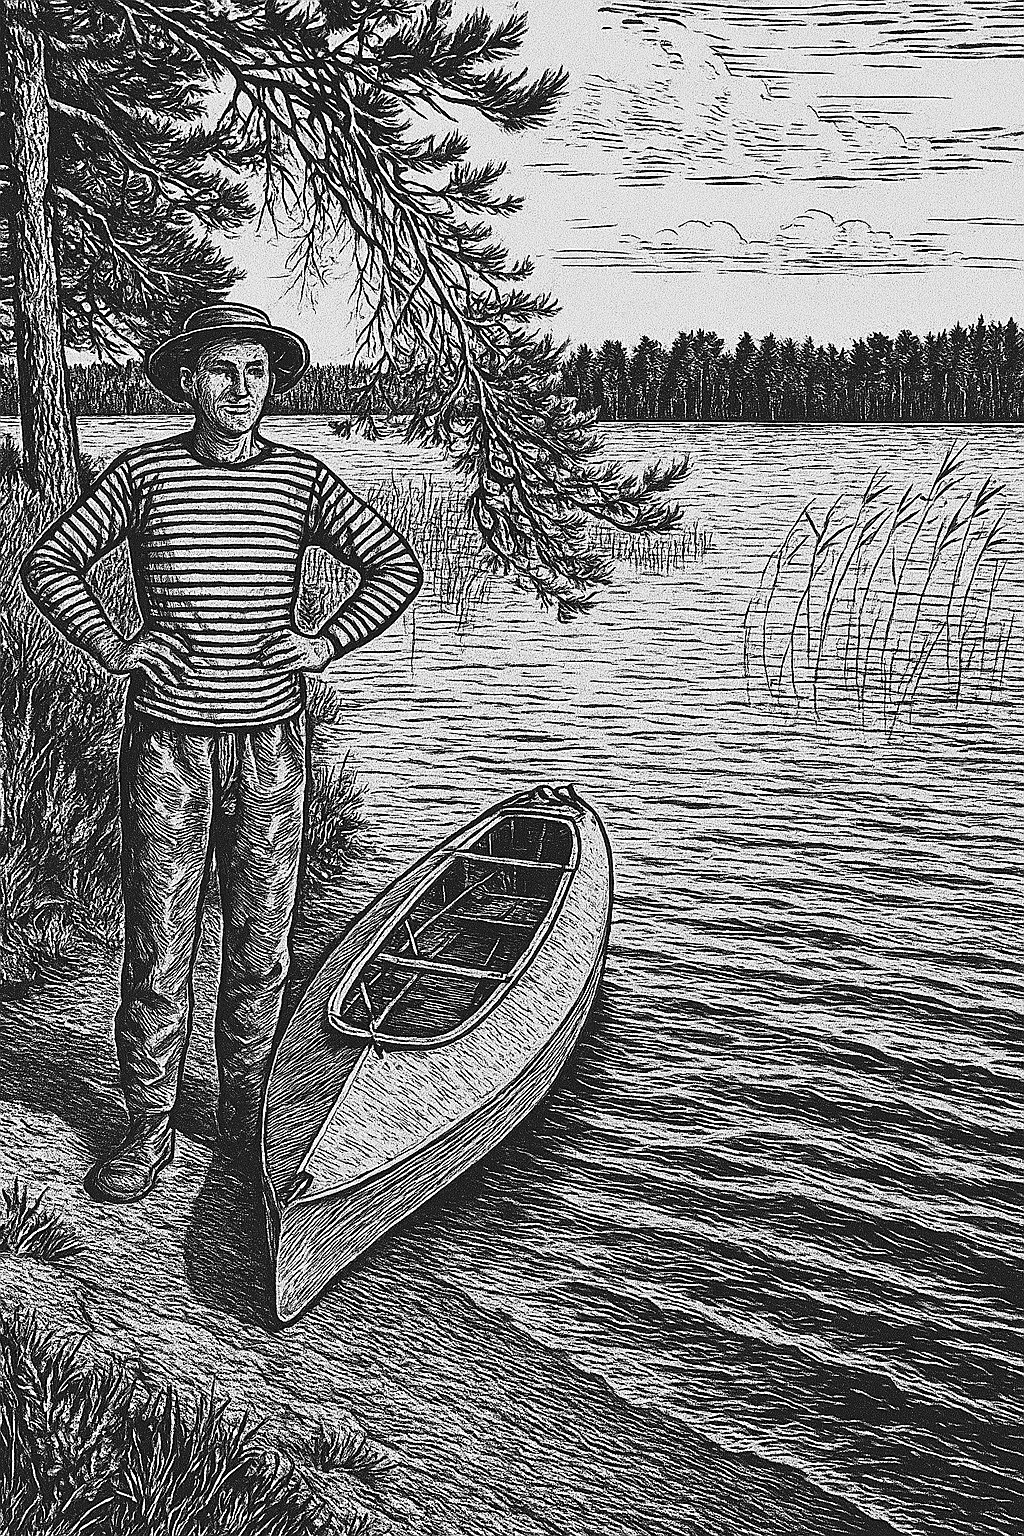
\includegraphics[width=1.0\textwidth]{9_4_new}
%	\caption{\small\textit{...пристали к берегу под сосной, росшей прям на берегу...}}
%\end{figure}

\begin{wrapfigure}[23]{l}{0.6\textwidth}
	%\begin{figure}[h]
	\centering
	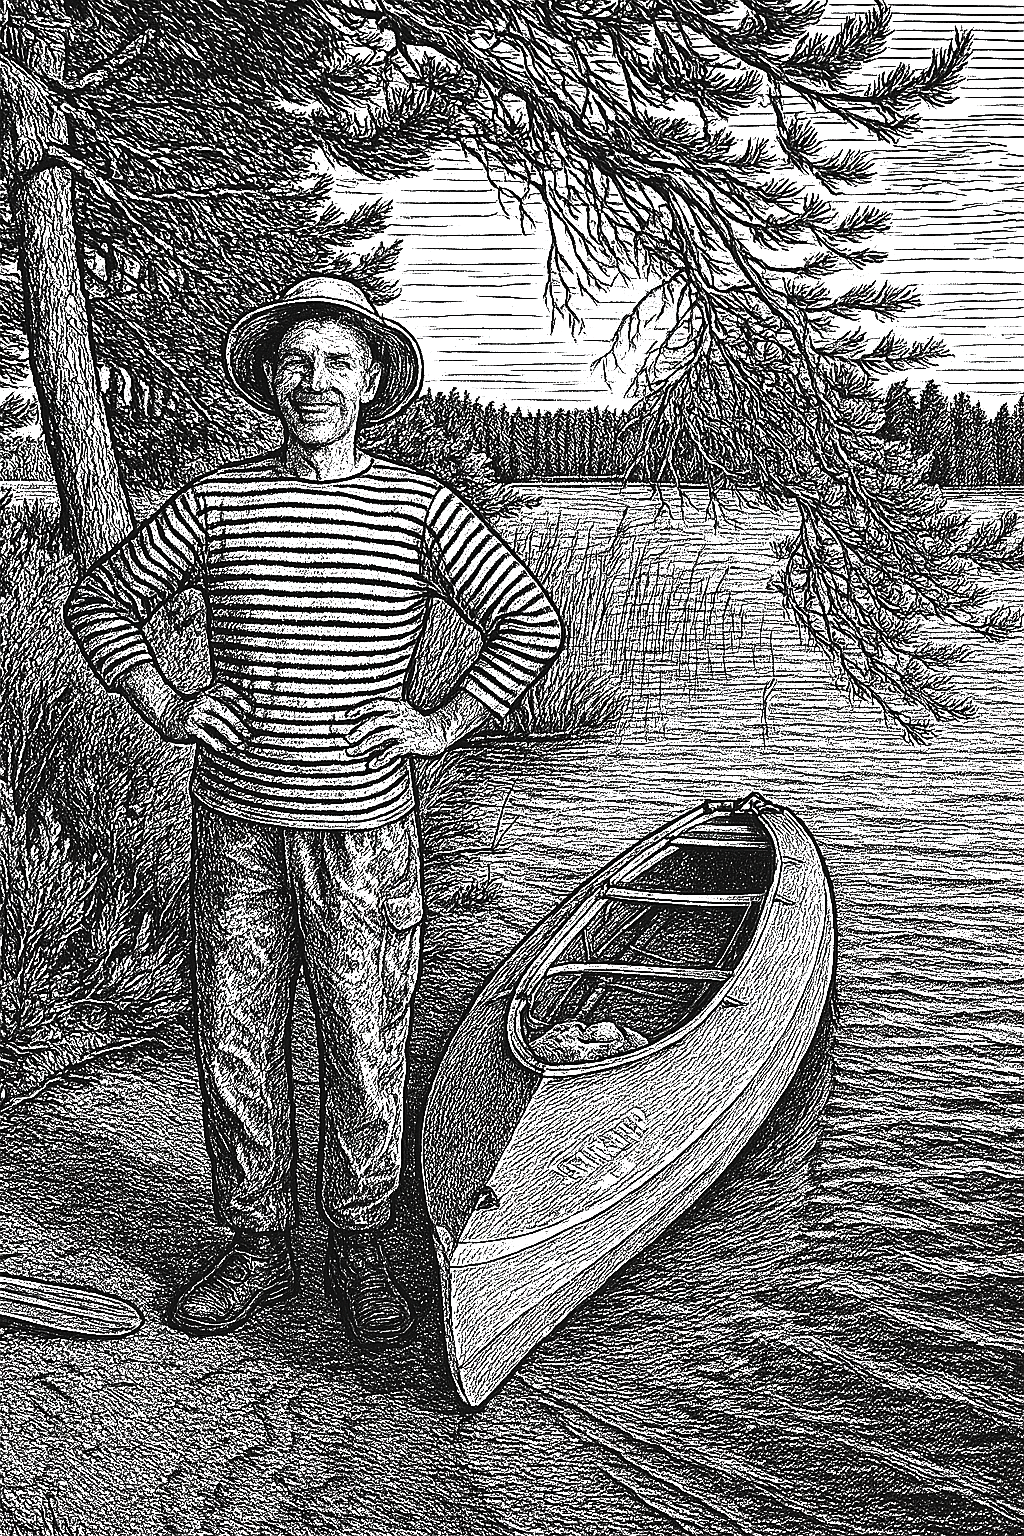
\includegraphics[width=0.6\textwidth]{27_1_shurik}
	\caption{\small\textit{...под сосной на берегу озера...}}
	%\end{figure}
\end{wrapfigure}

Вечер сгущался тёмный и~облачный. 
Над столом парни натянули тент, а к~соснам, росшим тут же, привалили гермы с продуктами и~вещмешки. 
%\begin{wrapfigure}[15]{l}{0.6\textwidth}
%\begin{figure}[h]
%	\centering
%	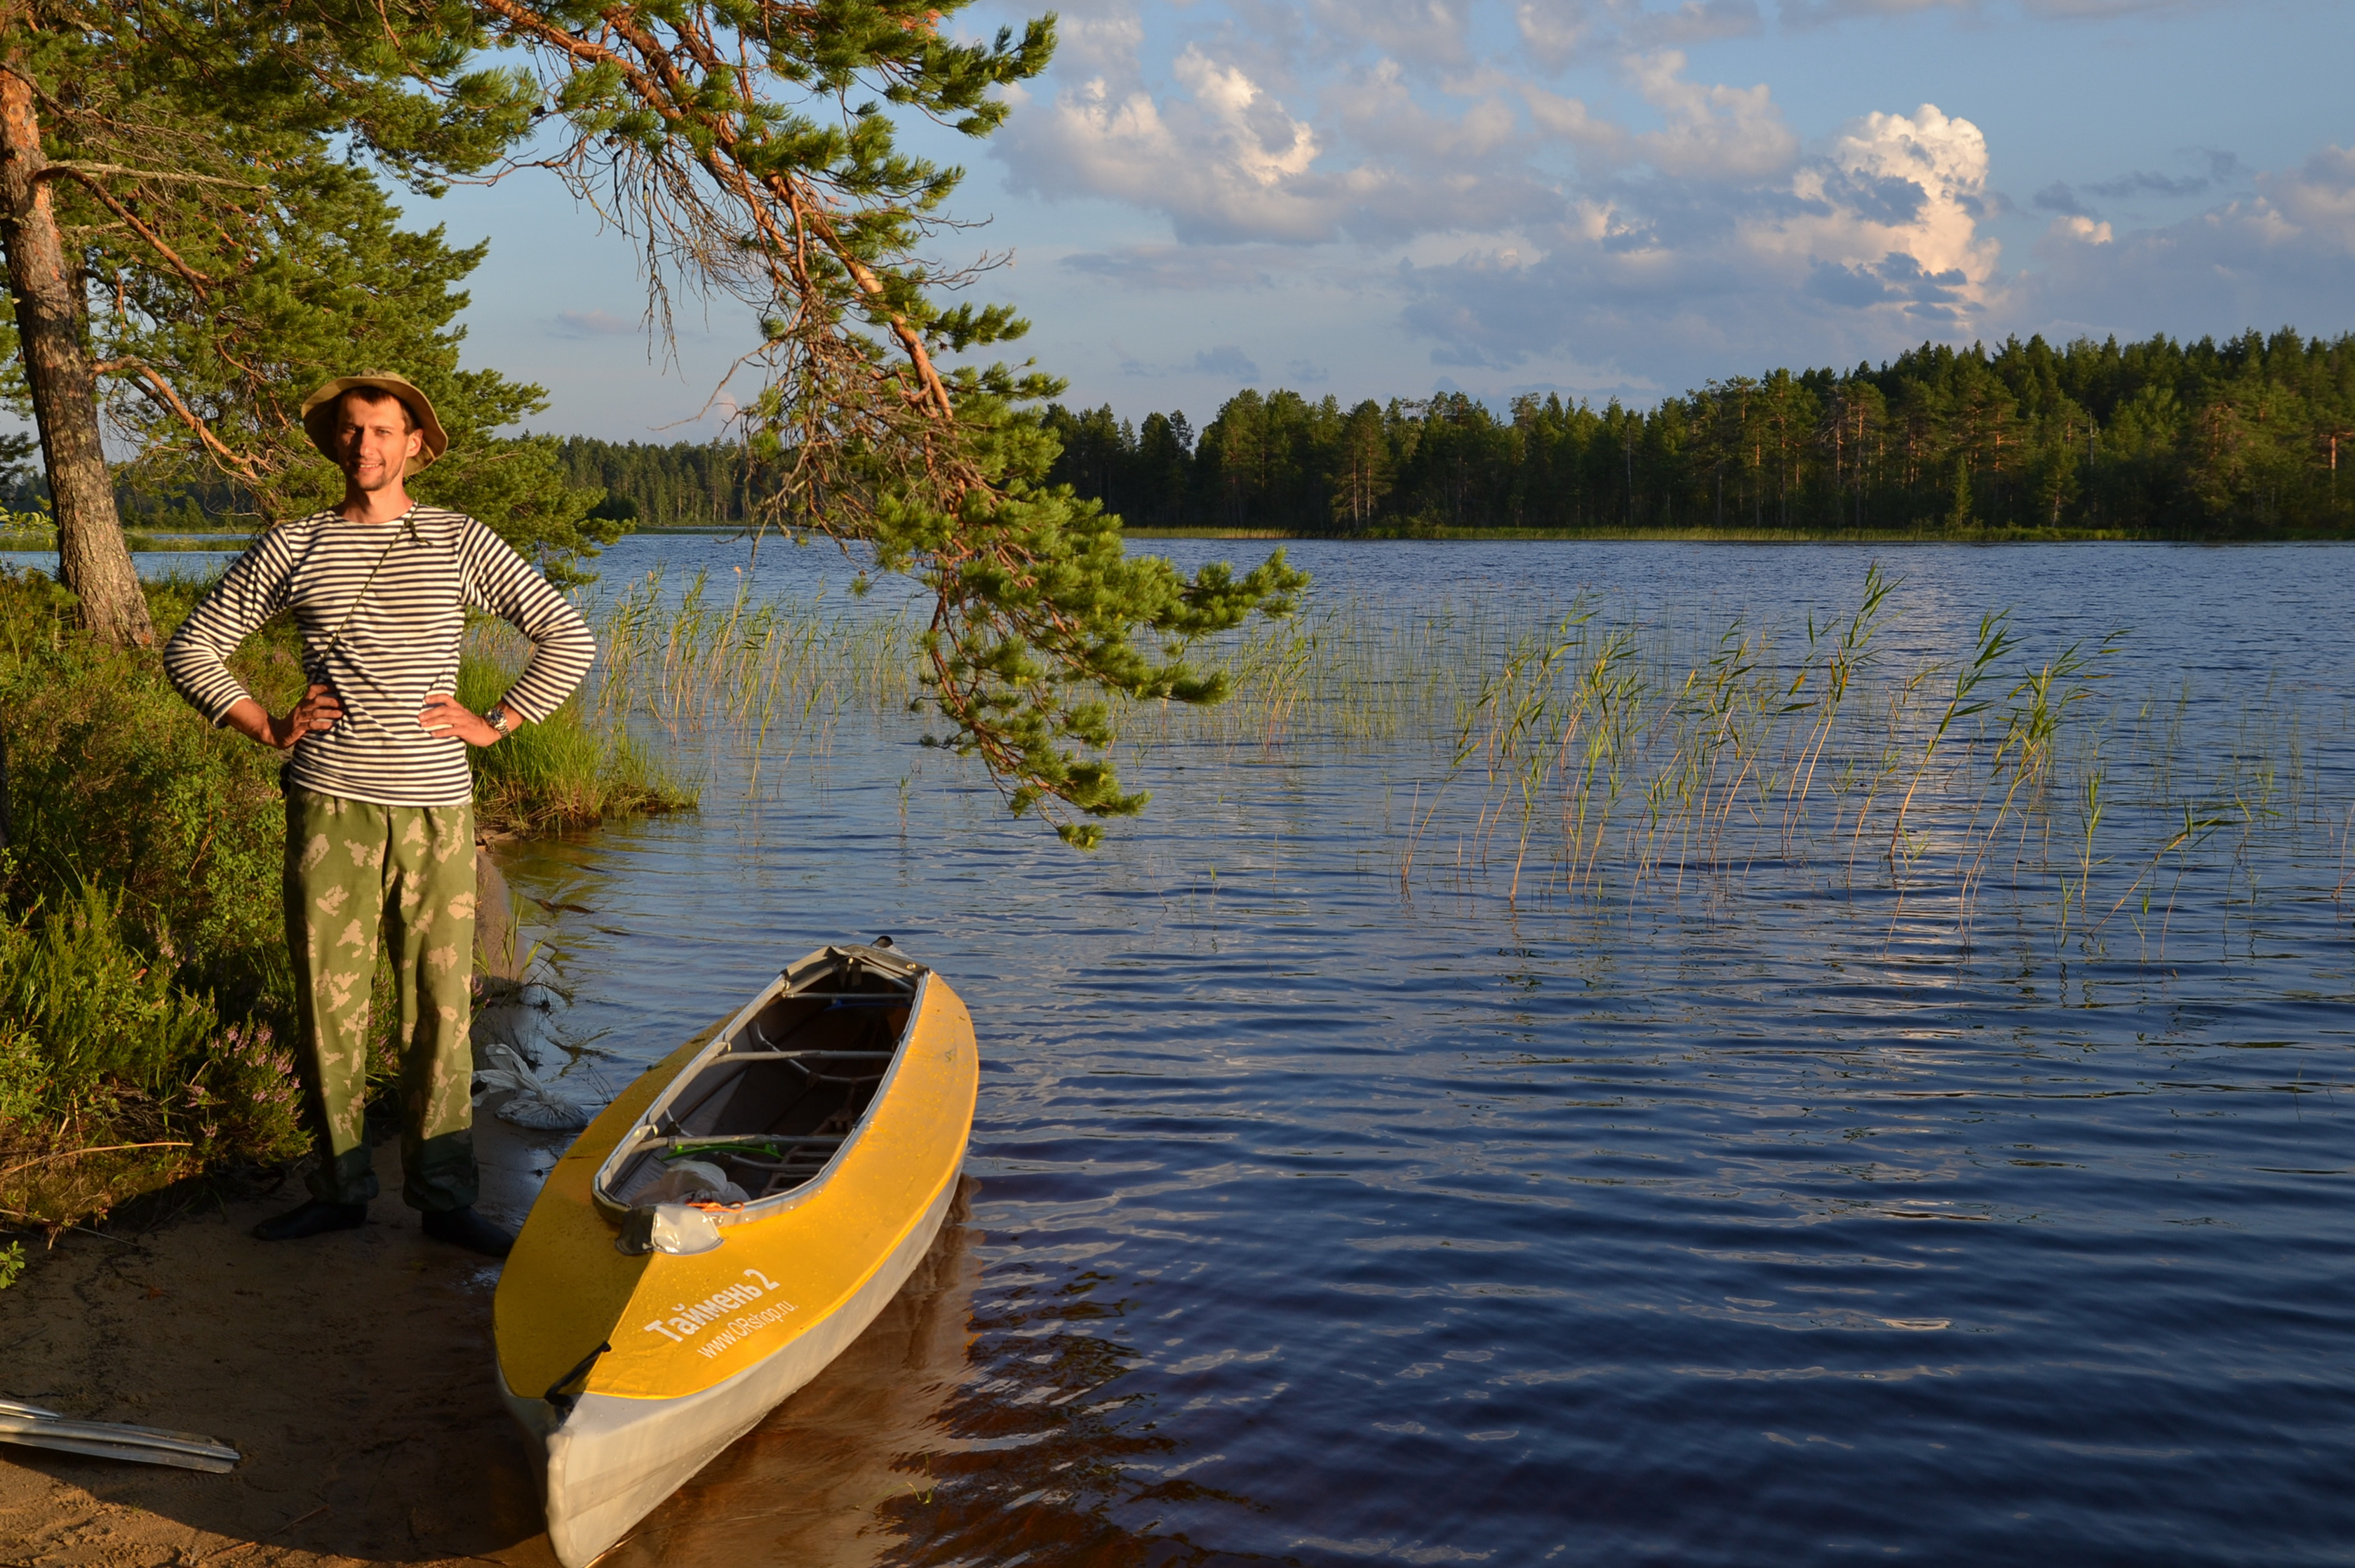
\includegraphics[width=1.0\textwidth]{9_4}
%	\caption{\small\textit{...пристали к берегу под сосной, росшей прям на берегу...}}
%\end{figure}
%\end{wrapfigure}
Костёр Адмирал мигом сообразил из имевшегося неподалёку валежника и отослал команду за нормальными дровами\mdash ему хотелось побыстрее сварить горячего.

Замполит~живо возглавил заготовку дров, дело спорилось\mdash у костра образовалась целая груда брёвен, что ребята притащили из леса. Котелки с водой уже пошумливали над костром, а Адмирал собрал свои походные кресла, уселся в~одно из них и распотрошил герму с~продуктами:

\diagdash Так, парни, что готовим?

\diagdash Суп понажористей!!!\mdash отозвался Замполит.

\diagdash Всегда п-жалста!\mdash Адмирал любил в походе готовить суп, который называл <<сырным>> из\sdash за добавления туда порезанного плавленного сырка <<Дружба>>. Сырок растворялся, и варево~получалось жирным и~питательным, причём совсем не важно, что за сухая покупная засыпка из~пакетика была в основе\mdash будь то <<вермишелевый суп>> или <<суп~с~говядиной>>, или <<харчо>>, или даже <<борщ>>\mdash после добавления плавленного сырка это было уже совершенно не важно, поскольку всё становилось одинаково сырным на~вкус.

Адмирал в темпе начистил картошки и поставил её вариться на суп, сделал заправку из лука и моркови. На~второе быстро отварили макароны и сдобрили их~тушёнкой. Быстро, да не быстро\mdash с момента причаливания уже прошло полтора часа\mdash они успели развернуть лагерь, поставить палатки, приготовить ужин. Настали сумерки. Паша, тем временем, подсуетился, притащил какой\sdash то пенёк, поставил сверху байдарочное сиденье, начистил лучок на закуску, нарезал хлеба, организовал сальца. Адмирал вытащил из~вещмешка очередной апельсин\mdash у~него было припасено по одной штуке на каждый день. Вкушать ужин они сели уже в~глубоких сумерках\mdash Адмирал с~Замполитом развалились в~раскладных креслах, Паша сбоку на складном стульчике, а~матросы с~другой стороны костра на поваленном бревне. Народ жадно уминал ужин, все проголодались.

\diagdash Денёк был угар$\ldots$\mdash Серёга звенел металлической ложкой по миске, наворачивая суп.%\mdash Скока мы сёдня прошли, Шурик, двадцать?

\diagdash Мужики, давайте, за начало днёвки!\mdash Адмирал поднял кружку.

\diagdash {\Large УРА, УРА, УРА\sdash А\sdash А!!!}

%\diagdash Ай, хорошо пошла!\mdash 
Замполит закусил и устало отвалился в кресло:

\diagdash Чуть не сдохли сегодня, блин.\mdash апельсин, сало и~лучок стремительно исчезали как закуска.

\diagdash Так чё, скока, говоришь, мы сёдня прошли, Шурик, двадцать?\mdash поинтересовался Серёга, доедая суп.

\diagdash Двадцать пять! Двадцать пять прошли сегодня по~GPS с учётом кругосветного, то есть кругоостровного плавания. Вполне себе стандартный километраж,\mdash Адмирал закусил апельсином, тоже развалившись в~походном кресле,\mdash мой рекорд\mdash сорок два километра на~Лиди в~2017\sdash м, так\sdash то!

\diagdash Ух, 25, ничё се!\mdash Серёга с Русланом удивились.

\diagdash И перекатов 6 или 7 прошли, да?\mdash Адмирал, естественно, угорал.

\diagdash Да како-о-ой! Три, по-моему!\mdash Серёга стал припоминать.\mdash Первый это типа мост был и стремнина за~ним, на втором мы с Кирей сели на камень и нас развернуло, а~последний мы пешкодралом шли!

\diagdash Как бурлаки на Волге, ы-ы-ы! Но самое главное, что никто,\mdash Адмирал поднял палец вверх,\mdash не пробился! И~встали на стоянку на острове посреди Линдозера. И,~в~принципе, неплохо, скажу я вам, встали. И за это вот всё надо бы эц\sdash самое$\ldots$

\diagdash Подставляй!\mdash ром лился рекой, еды и закуски у~них, как и~всегда, было предостаточно\mdash Адмирал уделял кулинарной части особое внимание.

Команда устала за день, переход дался им нелегко, подкосила внезапность, что ли, этих порогов, к которым никто не был готов, включая Адмирала. Но они без потерь всё преодолели и дошли, как и планировалось, до острова. Хоть~все и устали, у костра традиционно задержались, разговоры с каждым поднятием кружек текли оживлённее и оживлённее:

\diagdash Ну чё, как тебе поход наш?\mdash спросил Адмирал у~Руслана, уминая макароны.

\diagdash Класс! По озёрам так скучненько сначала было, а~по~порогам вообще по~кайфу!\mdash новичок неожиданно хорошо влился в их команду.

\diagdash Ага!\mdash согласились все.

\diagdash Дальше начнётся по\sdash настоящему активная часть маршрута\mdash пороги второй категории.\mdash напомнил команде Адмирал.

\diagdash На которые у нас нет описания, да?\mdash уточнил Серёга, надавив на больное, которое от этого менее актуальным не стало.

\diagdash Нету$\ldots$\mdash Замполит прикурил от костра.

\diagdash А чё, связь\sdash то есть? Кто\sdash нить смотрел мобильники?\mdash вспомнил Адмирал.

\diagdash Была одна <<палочка>> связи, да и пропала,\mdash Замполит достал телефон,\mdash надо завтра сходить на мыс, там попробовать половить связь.

\diagdash На мыс? Это к черноволосой?$\ldots$

\diagdash Ы-ы-ы!\mdash заржали парни.

\diagdash Ой не начинайте на ночь глядя!

\diagdash Ы-ы-ы!

\diagdash Так как раз на ночь\sdash то глядя и надо!

\diagdash Ы-ы-ы!

\diagdash Всё завтра, парни, сегодня уже просто некондиция.\mdash Серёга с Кирей устали больше всех, пока тащили байду на~последнем пороге.

\diagdash Что завтра делаем?\mdash спросил Руслан.

\diagdash Чилим, восстанавливаем силы, готовимся морально к настоящим порогам. А послезавтра с новыми силами выходим на активную часть маршрута. Руслан, как тебе в~целом походный быт? Уже на третий  день когда всё плюс\sdash минус устаканилось?\mdash Адмирал перешёл на чаёк со~сгущёнкой.

\diagdash Да так\sdash то ваще на чиле\mdash Серёга палатку сам ставит, ты готовишь. Грести особо не упахиваемся. Расслабончик с~элементами маленького экстрима, всё по кайфу!

\diagdash Ха, ну примерно да. Ну чё, орлы, наелись?

\diagdash От пуза, Шурик! Всё класс!

Они ещё с часок посидели у костра, наслаждаясь душистым чаем, в который добавили лимон. Разговоры текли всё менее оживлённо, все притомились. Кто потягивал чаёк с конфетами, кто смолил сигару, кто просто, развалившись в~стульчике, наслаждался ночным воздухом и~неповторимыми ароматами костра.

\diagdash Ладно, парни,\mdash Адмирал засобирался спать,\mdash я~просто валюсь с~ног!\mdash он залёг в палатку и~почти сразу же отрубился. Вокруг наступила пасмурная, но тихая и~спокойная карельская ночь.


%Вскоре все последовали его примеру и разбрелись по~своим палаткам, которые были тут же, поблизости на~полянке, и~поставлены. Наступила пасмурная, но тихая и~спокойная карельская ночь.
\vspace{-0.2cm}
\begin{center}
	\psvectorian[scale=0.4]{88} % Красивый вензелёк :)
\end{center}
